%%%%%%%%%%%%%%%%%%%%%%%%%%%%%%%%%%%%%%%%%%%%%%%%%%%%%%%%%%%%%%%%%%%%%%%%%%%
%
% Trabajo de fin de máster v1.0
% Guillermo Sánchez Brizuela
%
%%%%%%%%%%%%%%%%%%%%%%%%%%%%%%%%%%%%%%%%%%%%%%%%%%%%%%%%%%%%%%%%%%%%%%%%%%%

% Qué tipo de documento estamos por comenzar:
\documentclass[a4paper]{article}
% Esto es para que el LaTeX sepa que el texto está en español:
\usepackage[spanish,es-tabla]{babel}
\selectlanguage{spanish}
% Esto es para poder escribir acentos directamente:
\usepackage[utf8]{inputenc}
\usepackage[T1]{fontenc}
% Para texto tachado
\usepackage[normalem]{ulem}
% Imágenes en el lateral
\usepackage{wrapfig}
% Tablas
\usepackage{booktabs}
% Anexos
\usepackage{appendix}
%Tablas
\usepackage{float}
% Leyendas
\usepackage{caption}
\captionsetup{justification=centering}
% Bibliografia en la tabla de contenidos
\usepackage[nottoc,notlot,notlof]{tocbibind}
% Tablas
\usepackage{booktabs}
\usepackage[table,xcdraw]{xcolor}


% Definición de un nuevo comando
\newcommand{\textbfit}[1]{\textbf{\textit{#1}}}



%% Asigna un tamaño a la hoja y los márgenes
\usepackage[a4paper,top=3cm,bottom=2cm,left=2.5cm,right=2.5cm,marginparwidth=2cm]{geometry}

%% Paquetes de la AMS
\usepackage{amsmath, amsthm, amsfonts}
%% Para añadir archivos con extensión pdf, jpg, png or tif
\usepackage{graphicx}
\usepackage[colorinlistoftodos]{todonotes}
\usepackage[colorlinks=true, allcolors=blue]{hyperref}
%% Simbolo de grado
\usepackage{gensymb}
%% Imágenes en vertical
\usepackage{subfig}
\usepackage{graphicx}

\usepackage{nomencl}
\makenomenclature
\nomenclature{Estática}{(Imagen) Capturada o generada de forma individual y no como parte de un vídeo.}
\nomenclature{Vídeo}{Sucesión de imágenes continua que aporta ilusión de movimiento.}
\nomenclature{Online}{(Procesamiento) Que ocurre a medida que llega nueva información.}
\nomenclature{Offline}{(Procesamiento) Que trabaja sobre información previamente recogida.}
\def\nomname{Terminología}

%% Primero escribimos el título
\title{Borrador TFM/Memoria de prácticas: Estimación de Profundidad Monocular Online con Transformers Eficientes}
\author{Guillermo Sánchez Brizuela\\
  \small Universidad de Valladolid\\
  \small Valladolid, España
  \date{}
}

%% Después del "preámbulo", podemos empezar el documento

\begin{document}

\begin{titlepage}
\centering
\begin{figure}[t]
	\centering
	
\includegraphics[scale=0.35]{imagenes/gsi.png}
    \vspace{0.5cm}
\end{figure}%
	{\LARGE Memoria del trabajo realizado durante la estancia en el Grupo de Sistemas Inteligentes\par}
	\vspace{3cm}
	{\huge\bfseries Estimación de Profundidad Monocular Online con Transformers Eficientes\par}
	\vspace{0.5cm}
    {\LARGE Contexto y estado del arte\par}
    \vspace{3cm}
	{\Large\itshape Guillermo Sánchez Brizuela\par}
	\vspace{0.5cm}
	{\Large Universidad de Valladolid, curso 2020-2021\par}
	\vfill
\end{titlepage}

%% Imprimimos la nomenclatura
% \todo[inline]{Repasar las definiciones.}
% \printnomenclature[3cm]

%% Tabla de contenidos
{
    \setcounter{tocdepth}{4}
    \setcounter{secnumdepth}{4}
    \hypersetup{linkcolor=black}
    \tableofcontents
}

\newpage

%% Hay que decirle que incluya el título en el documento
% \maketitle

%% Aquí podemos añadir un resumen del trabajo (o del artículo en su caso) 
% \begin{abstract}
% Lorem ipsum.
% \end{abstract}

% \todo[inline]{Hacer portada y buscar normas del tfm. (TFM)}
%% Iniciamos "secciones" que servirán como subtítulos
\section{Introducción}
Al capturar a través de una cámara una imagen o un vídeo, se proyecta en dos dimensiones una realidad tridimensional, perdiendo así la información relativa a la profundidad de la escena. Existen soluciones hardware que capturan escenas tridimensionales sin perder ninguna dimensión, por ejemplo, los LiDAR, las cámaras de tiempo de vuelo o conjuntos de cámaras para estereovisión\footnote{Con una pareja de cámaras con posiciones conocidas, es posible estimar la profundidad a partir de la disparidad geométrica entre las dos imágenes capturadas.}. Sin embargo, recuperar la profundidad de una imagen obtenida con una cámara corriente sigue siendo un problema cuya solución sería de gran utilidad:
\begin{itemize}
    \item En distintos campos como la robótica/conducción autónoma (navegación, odometría visual, etc.), la realidad aumentada, la generación de modelos 3D, etc.
    \item Como información de apoyo en otras tareas típicas de la visión artificial (detección, segmentación, clasificación).
\end{itemize}

Pese a haberse estudiado extensamente, la estimación de profundidades aún está lejos de ser resuelta por completo. Dentro de las técnicas que se han desarrollado y probado a lo largo de los años, tanto dentro de la visión artificial en general como en concreto para la estimación de profundidades, destacan aquellas que se basan en aprendizaje automático debido a su alta capacidad para trabajar en nuevas situaciones desconocidas previamente y bajo condiciones donde las técnicas de visión artificial tradicionales sufren ya que ocurren cambios significativos en la iluminación, los colores y/o orientaciones. 

Este trabajo, resultado de la asignatura I+D+i en Informática del máster en Ingeniería Informática desarrollada en el Grupo de Sistemas Inteligentes, se centra en estudiar y revisar aquellas propuestas para estimar profundidades basadas en aprendizaje automático, en especial las que emplean \textit{transformers}, así como las técnicas existentes para acelerar su inferencia.

\subsection{Motivación}
El campo del aprendizaje automático progresa a un ritmo considerablemente difícil de seguir (34736 publicaciones relacionadas con aprendizaje automático en arXiv en el año 2020 \cite{ai_index_report_2021}). Por esto, surge la necesidad de un documento que recoja los distintos enfoques relacionados con la estimación de profundidades basados en aprendizaje automático en conjunto con las técnicas que permiten ejecutar estos modelos de forma online (entendiendo por online el procesamiento de las entradas a medida que llegan, pero sin las restricciones propias de un entorno de tiempo real).

Además de esto, parte de la motivación de este documento viene dada por el trabajo de fin de máster que se realizará como continuación de este trabajo. Este trabajo, consistirá en la modificación de uno de los modelos basados en \textit{transformers} y aprendizaje supervisado para inferir resultados en equipos con recursos de computación limitada de forma online. En este caso, los equipos con recursos de computación limitada serán equipos de nivel consumidor o dispositivos embebidos con hardware especializado.

%% \textbf{(TFM)} Lorem ipsum

\subsection{Objetivos}
Los objetivos definidos para este periodo de prácticas, y por lo tanto aquellos en los que se centra este documento son los siguientes:
\begin{enumerate}
    \item Revisión del estado del arte relacionado con la estimación de profundidades empleando técnicas de aprendizaje automático, con especial hincapié en aquellas donde se emplean \textit{transformers}.
    \item Revisión de distintos métodos, tanto especializados en \textit{transformers} como generales, que aceleren entrenamiento e inferencia y reduzcan el tamaño de los modelos.
    \item Realización de distintas pruebas de rendimiento y comparación de resultados entre distintas arquitecturas del estado del arte actual de estimación de profundidades dentro del aprendizaje supervisado empleando \textit{transformers}.
\end{enumerate}

\clearpage
% \textbf{(TFM)} Lorem ipsum

\section{Plan de trabajo}
El plan de trabajo inicial destinaba aproximadamente la mitad de las horas de la estancia a la realización de \textit{benchmarks} sobre los distintos modelos existentes para estimación de profundidades. Sin embargo, con el trabajo de la primera semana, que sirvió para contextualizar el problema, se comprobó que las soluciones existentes eran demasiado numerosas y variadas como para compararlas sistemáticamente entre sí. Por lo tanto, la planificación pasó a centrarse en la elaboración de una base de conocimiento suficientemente sólida con la que ajustar el enfoque del trabajo de fin de máster. Esta segunda planificación, ha sido controlada y modificada semanalmente en las reuniones semanales con el tutor donde se han presentado resultados parciales, resultando de la siguiente manera. 

\begin{figure}[H]
\centering
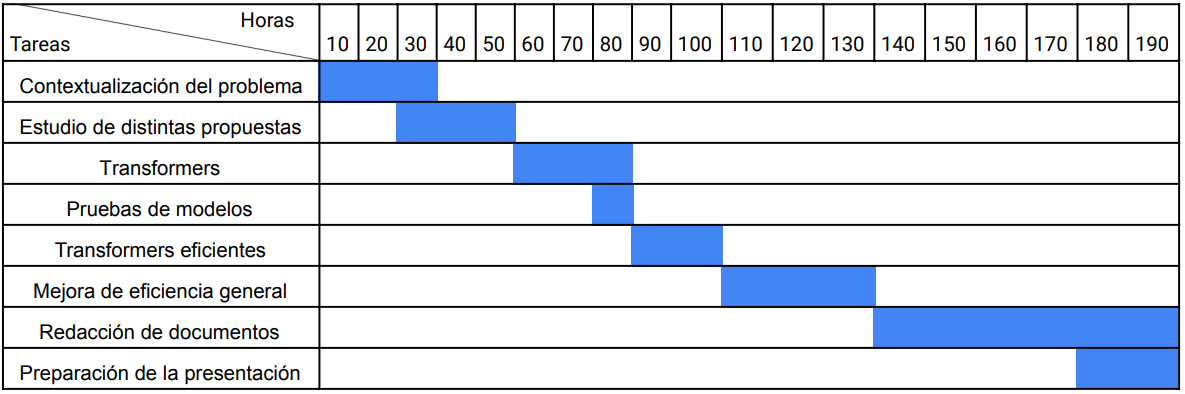
\includegraphics[width=0.95\linewidth]{imagenes/planificacion_horaria.png} 
%\caption{Planificación horaria.}
\label{fig:planificacion-horaria}
\end{figure}

\section{Resultados obtenidos}
Este ha sido principalmente un trabajo de revisión bibliográfica, cuyo objetivo era construir una base de conocimiento sobre la estimación de profundidades en imágenes monoculares con un cierto enfoque en las técnicas (tanto generales como específicas) capaces de acelerar dichos modelos. Por lo tanto, los resultados se presentan resumidos en el capítulo \ref{marco_teorico_estado_arte} en forma de marco teórico y estudio del estado del arte. Además de este estudio, se incluyen también en el capítulo \ref{resultados} los resultados de las pruebas de velocidad de inferencia que se han realizado en algunos de los modelos. Estas pruebas, tienen como objetivo comprobar la capacidad de modelos concretos para inferir resultados de forma online en diferente \textit{hardware}.

\section{Marco teórico y estado del arte}\label{marco_teorico_estado_arte}

Dado que este trabajo se centra en los modelos basados en \textit{transformers}, una arquitectura de red neuronal relativamente nueva (2017), se describen primero estas arquitecturas.

\subsection{Redes neuronales - Transformers}
La arquitectura inicial del \textit{transformer} (Figura \ref{fig:arquitectura-transformer}), propuesta en \textit{Attention is All You Need} \cite{NIPS2017_3f5ee243}, se basa en una estructura \textit{encoder-decoder}. Es decir, un conjunto de capas (\textit{encoder}) que codifica la entrada en una representación latente, que después es tomada como entrada del \textit{decoder}, otro conjunto de capas que decodifica esta representación latente en una salida útil. En la propuesta inicial, destinada a procesamiento de lenguaje natural, el \textit{encoder} se encarga de trasladar una secuencia de entrada $(x_1, ..., x_n)$ - una frase - en una secuencia de representación $(z_1, ..., z_n)$. Esta secuencia $z$, es la entrada del \textit{decoder}, que la convierte en una secuencia de salida $(y_1, ..., y_m)$ - otra frase -. Una de las principales diferencias frente a los modelos \textit{encoder-decoder} basados en redes recurrentes, es que a pesar de que el modelo sigue siendo auto-regresivo, es decir, sigue utilizando los elementos generados por la salida del modelo como entrada para el siguiente elemento a generar, en este caso la secuencia de entrada no está alineada temporalmente con la ejecución del modelo y por lo tanto puede paralelizarse todo el procesamiento de dicha secuencia, acelerando entrenamiento e inferencia.
% Las redes recurrentes, especialmente aquellas que emplean celdas LSTM \cite{HochSchm97} y GRU \cite{cho-etal-2014-learning}, son modelos establecidos como estándar a la hora de trabajar con secuencias, sin embargo, 
% \todo[inline]{Hilar con las redes recurrentes para compararlo después con ellas.}

% \paragraph{Arquitectura}\mbox{}
\clearpage
\subsubsection{Arquitectura}

\vspace{2mm}

\begin{wrapfigure}{r}{0.5\textwidth}
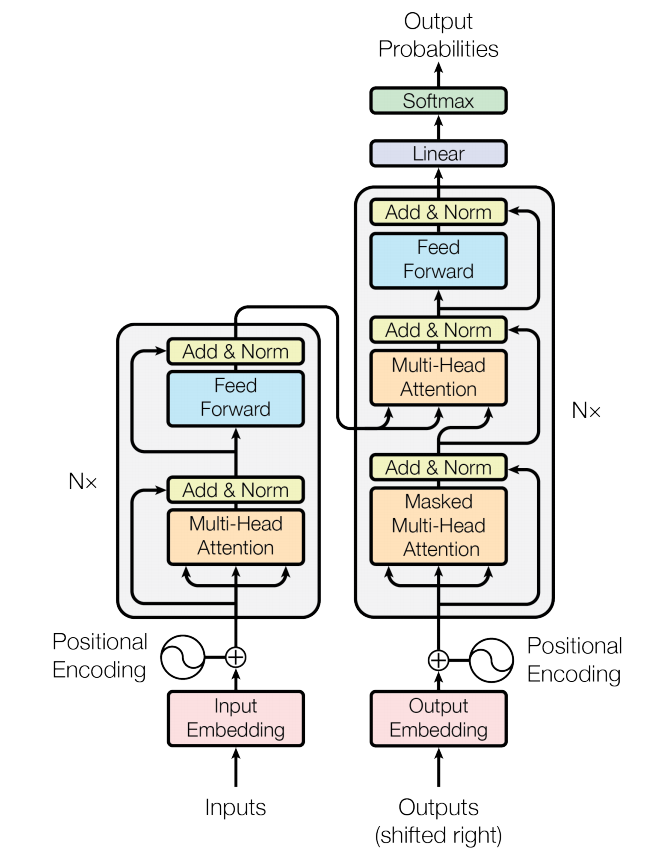
\includegraphics[width=0.95\linewidth]{imagenes/transformer-arquitectura.png} 
\caption{Arquitectura del \textit{transformer}.\\Fuente: \cite{NIPS2017_3f5ee243}}
\label{fig:arquitectura-transformer}
\end{wrapfigure}

\vspace{2mm}
En el \textbf{encoder} (parte izquierda de la Figura \ref{fig:arquitectura-transformer}), se encuentra un \textit{stack} de 6 capas. Cada una de estas, está compuesta por dos subcapas: una capa de \textit{Multi-Head Self-Attention} (un mecanismo de atención que se explicará más adelante); y una capa que contiene una red \textit{feed-forward} totalmente conectada. Cada una de estas subcapas, cuenta además con una conexión residual, que conecta la entrada de la subcapa con su salida de forma que puedan ser sumadas y normalizadas. Para facilitar la suma y normalización de entradas y salidas, todas las capas del modelo producen elementos de dimensión $d=512$. Antes de estas 6 capas, cada uno de los \textit{tokens} - elementos de la secuencia - de entrada (en la propuesta inicial, palabras), se convierten a vectores de dimensión $d$ a través de un \textit{embedding}\footnote{Operación que transforma, en el caso de la publicación original, palabras, en una representación numérica en un espacio vectorial donde las palabras con significado similar se encuentran próximas entre sí} previamente entrenado y se les añade una codificación posicional (en esta propuesta, generada a partir de funciones seno y coseno de distintas frecuencias) que aporta al modelo información sobre la posición de cada \textit{token} dentro de la secuencia inicial.

\vspace{2mm}
Por otro lado, en el \textbf{decoder} (parte derecha de la Figura \ref{fig:arquitectura-transformer}), se vuelve a encontrar un \textit{embedding} previamente entrenado que transforma las salidas del modelo desplazadas una posición. Al resultado de este \textit{embedding}, se le añade una codificación posicional similar a la del \textit{encoder}. A continuación, hay otro \textit{stack} de 6 capas, que esta vez está compuesto por las dos subcapas que están presentes en el \textit{encoder} (en este caso la capa de \textit{Multi-Head Self-Attention} es en realidad \textit{Multi-Head Masked Self-Attention} ya que se aplica una máscara para evitar que influyan en la red los \textit{tokens} siguientes al \textit{token} que se va a predecir), y una subcapa adicional de \textit{Multi-Head Cross-Attention}, situada entre las otras dos subcapas, donde las salidas de la subcapa de \textit{masked self-attention} del \textit{decoder} pueden acceder a las salidas del conjunto de capas del \textit{encoder}. (\textbf{La entrada de esta última capa de atención proviene de la última capa del \textit{encoder}, no de sus capas intermedias}). Por último, a la salida del \textit{stack} de capas del \textit{decoder}, se encuentra una transformación lineal (entrenada) y una función softmax para predecir la salida de la red.

% \paragraph{Mecanismos de atención}\mbox{}\\
\subsubsection{Mecanismos de atención}
% \todo[inline]{Hablar de los mecanismos de atención, y aunque se mencionen sus comienzos y sus aplicaciones en redes recurrentes y convolucionales, centrarse en que son la principal baza de los transformers y su "novedad", ya que solo funcionan con esto básicamente, si queda muy pegado aquí se puede sacar como subapartado de Redes Neuronales y distintas topologías.}

\vspace{2mm}
Los mecanismos de atención, presentados por primera vez en \cite{neuralmachinetranslationalignandtranslate}, buscan simular la atención cognitiva y han sido previamente empleados en redes recurrentes \cite{pmlr-v37-xuc15} y convolucionales \cite{7298685, 7410695} para aprender qué partes de la entrada son más relevantes en la tarea a completar. Sin embargo, en \cite{NIPS2017_3f5ee243}, con los \textit{transformers}, se propone por primera vez una arquitectura basada solamente en estos mecanismos. 
% \sout{De esta forma, se eliminan los sesgos cognitivos \cite{} que se han introducido en arquitecturas anteriores para facilitar su aprendizaje y mejorar su funcionamiento. Dichos sesgos cognitivos, son, por ejemplo, el uso de convoluciones para tratamiento de imágenes, donde se presupone que los elementos más cercanos a un píxel serán de mayor interés; o el uso de redes recurrentes secuenciales para procesamiento de lenguaje natural, donde se almacena toda la información que precede a un elemento de forma conjunta.} 
Las funciones de atención más empleadas son la atención aditiva \cite{neuralmachinetranslationalignandtranslate} y multiplicativa, siendo esta última la empleada en los \textit{transformers}, donde la atención se consigue a través de un producto escalar dentro de un bloque con múltiples cabezas llamado \textit{Multi-Head Attention}, elementos principales de los \textit{transformers}, que aparecen de dos formas distintas:
\begin{itemize}
    \item Bloques de \textit{Self-Attention}, en el \textit{encoder} y en el \textit{decoder}, con todas las entradas dentro de sus respectivas capas.
    \item Bloques de \textit{Cross-Attention}, en las capas del \textit{decoder}, con entradas provenientes del final de la pila de capas del \textit{encoder} y de la subcapa anterior del \textit{decoder}.
\end{itemize}
Cada una de las cabezas que componen estos bloques basan su funcionamiento en multiplicar sus entradas por una serie de matrices $W^V$, $W^K$ y $W^Q$ que son aprendidas durante el entrenamiento, de donde se obtienen, respectivamente, vectores \textit{Value} (V), \textit{Key} (K) y \textit{Query} (Q). Estos vectores, permiten que cada uno de los elementos de la secuencia de entrada, con el cálculo asociado a la atención (Figura \ref{fig:multi-head-attention}) soliciten a través de su vector \textit{Query} la información que determinen más importante de la secuencia. Esto se consigue al calcular el producto escalar de todos los vectores Q con todos los vectores K, que resultará mayor cuanto más alineados estén ambos vectores - mayor similitud entre las \textit{Queries} (consultas) y las \textit{Keys} (claves) -. A los resultados de estos productos escalares, se les aplica una función \textit{SoftMax} para asegurar que sumen una unidad y finalmente se multiplican por los vectores V para obtener el resultado final de la atención. Los resultados de todas las cabezas, se concatenan en una sola matriz para aprovechar al máximo el procesamiento en paralelo y atraviesan una última proyección linear.
% \todo[inline]{Hablar de la operación de atención y de como permite que se configuren los pesos automáticamente y acabar lo de softmax}
% \todo[inline]{En el anexo 1, hacer algo similar a \url{https://youtu.be/4Bdc55j80l8} + \url{https://jalammar.github.io/illustrated-transformer/}}
\begin{figure}[H]
\centering
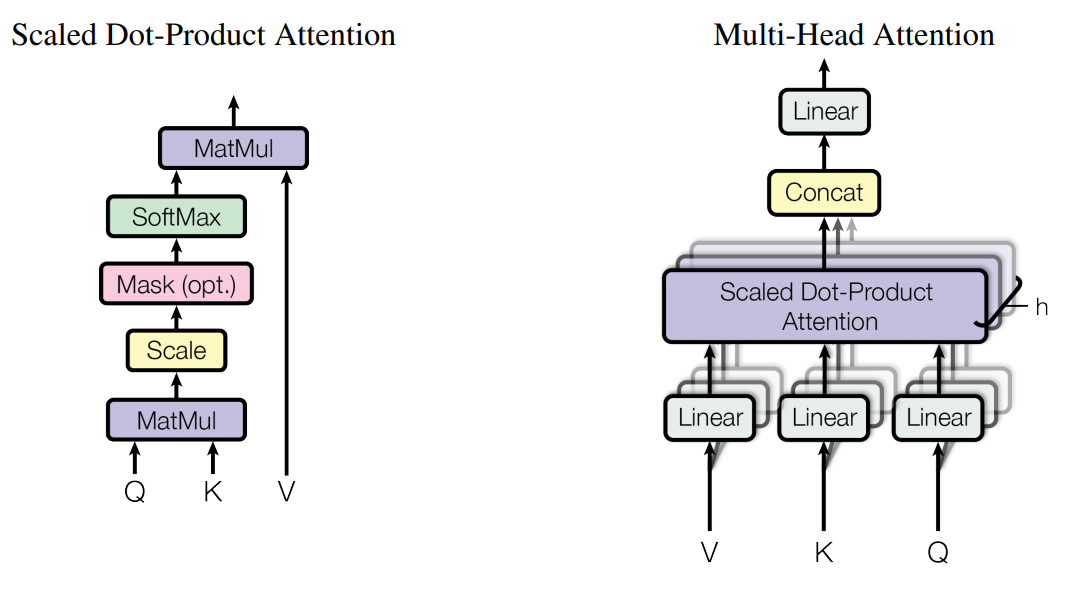
\includegraphics[width=0.65\linewidth]{imagenes/multi-head-attention.png} 
\captionsetup{width=.8\linewidth}
\caption{Producto escalar para el cálculo de la atención (izquierda) y bloque de \textit{Multi-Head Attention} (derecha). Fuente: \cite{NIPS2017_3f5ee243}}
\label{fig:multi-head-attention}
\end{figure}

% Estos mecanismos de atención, sin embargo, son costosos, ya que tienen una complejidad $O(n^{2})$ tanto en tiempo como en memoria, siendo n el número de elementos de la secuencia de entrada (al bloque de atención). Es por esto por lo que han ido surgiendo una serie de propuestas para reducir dicha complejidad computacional, algunas de las cuales se exponen en la sección \hyperref[transformers-eficientes]{Transformers eficientes}.

%\paragraph{Transformers para visión}\mbox{}
\subsubsection{Transformers para visión}

A la hora de aplicar la arquitectura de los \textit{transformers} a problemas de tratamiento de imágenes, surge un problema importante. La complejidad del mecanismo de atención es $O(n^{2})$, siendo n el número de elementos en la secuencia de entrada, por lo que para una imagen de dimensiones $lado \times lado$, el número de píxeles que conformarían la secuencia de entrada al mecanismo de atención es $n = l^2$, disparando la complejidad de la atención a $O(l^{4})$. Para lidiar con este problema, se han propuesto distintas soluciones como limitar el mecanismo de atención al entorno de cada píxel (presentado en \textit{Image Transformers} \cite{image_transformer}) o aplicar convoluciones para reducir el tamaño de la secuencia de entrada \cite{detrfacebookdetectiontransformers}. 

Sin embargo, la solución propuesta en \textit{An Image is Worth 16x16 Words} con el \textit{Vision Transformer} \cite{image16x16words} es la que mejores resultados ha obtenido y por lo tanto aquella que más popularidad ha ganado como base de arquitecturas para otros problemas de visión artificial \cite{visiontransformersDPT, bhat2020adabins, chen2021transunet, liu2021Swin}. Esta solución, consiste en dividir la imagen original en fragmentos de tamaño fijo y convertir con una proyección cada fragmento en un vector de valores (\textit{embedding}). Estos vectores, son equivalentes al resultado del \textit{embedding} de palabras en la arquitectura original y se introducen al modelo como tal, es decir, cada fragmento extraído de la imagen correspondería a una palabra de una frase (Figura \ref{fig:vision-transformer}). Como nota, esta arquitectura, inicialmente propuesta para realizar clasificación, solamente emplea el \textit{encoder} del \textit{transformer}.

\begin{figure}[H]
\centering
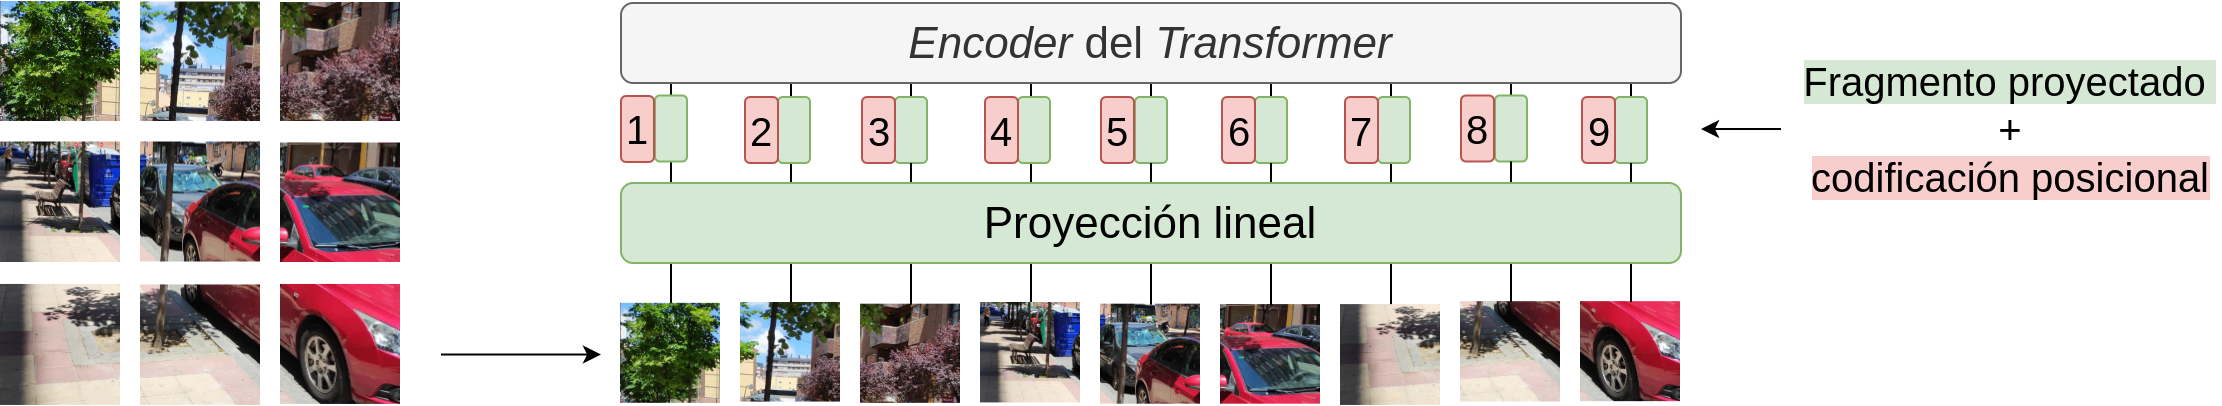
\includegraphics[width=1\linewidth]{imagenes/vision-transformer.png} 
\captionsetup{width=.8\linewidth}
\caption{Separación de una imagen en fragmentos siguiendo la propuesta de \cite{image16x16words}. Fuente: Elaboración propia inspirada en \cite{image16x16words}}
\label{fig:vision-transformer}
\end{figure}

% \todo[inline]{Esto es susceptible de moverse a la sección de estado del arte, se podría introducir las técnicas generales sin centrarnos en los papers.}


% \subsubsection{Mecanismos? de eficiencia} \label{eficiencia-general}

\subsection{Estimación de profundidades}
La estimación de profundidades, tanto cuando es llevada a cabo por humanos como por máquinas, consiste en detectar la distancia relativa entre todo aquello que se ve. Para conseguir esto, nuestro cerebro se apoya principalmente en la disparidad existente entra las imágenes que capturan cada uno de nuestros ojos, ya que las cosas que están más lejanas ven su posición menos alterada entre la vista de un ojo y de otro que las cosas cercanas. Esto se conoce como estereovisión.

Si nos tapamos un ojo, deberíamos perder esta capacidad para percibir la profundidad, sin embargo, esto no ocurre debido a que el cerebro explota lo que se conocen como pistas monoculares, que aportan información sobre la distancia a la que están las cosas a partir de las oclusiones, sombras, perspectiva, el tamaño esperado de un objeto, el paralaje, etc.

Las técnicas de visión artificial tradicional (basadas en dos cámaras - visión estereoscópica) no pueden lidiar con este problema, por lo que la estimación monocular (con una sola cámara) es prácticamente imposible. Para este tipo de estimación (monocular), entran en juego los modelos de aprendizaje automático, que han demostrado una gran capacidad para explotar este tipo de construcciones en todo tipo de tareas, no siendo la estimación de profundidades diferente. No obstante, a continuación se enumeran los distintos enfoques existentes, tanto tradicionales como basados en aprendizaje automático, en los cuales se profundizará especialmente.

% \todo[inline]{Hablar de la estimación de profundidades desde un punto de vista general, explicar por qué es un problema hacerlo con solo una cámara, por qué es interesante resolver este problema, qué utilidades puede tener, etc.}
% \todo[inline]{Contar un poco cómo usamos estereovisión y las pistas monoculares, se puede mover también al contexto/motivación de la introducción.}

% \subsection{Redes neuronales y distintas topologías}
% \todo[inline]{Hablar brevemente de las redes neuronales, en las subsecciones, hablar, de más a menos, de transformers > convolucionales > recurrentes.}

% \subsubsection{Redes convolucionales}
% Lorem ipsum
% \subsubsection{Redes recurrentes}
% Lorem ipsum
% \subsubsection{Transformers}

\subsubsection{Técnicas de estimación de profundidades} \label{estimacion-profundidades-sota}

La estimación de profundidades se ha intentado resolver de múltiples maneras \cite{Zhao_2020}. Dentro de estas metodologías, existen tres enfoques principales en función del tipo de \textit{software} o \textit{hardware} que se emplea.
\begin{itemize}
    \item \textbf{Soluciones geométricas}: Este grupo de métodos, extrae información de las restricciones geométricas que existen entre parejas de imágenes. Principalmente se agrupan en técnicas de \textit{SfM (Structure from Motion}) donde se reconstruye la tercera dimensión a partir de imágenes tomadas por una sola cámara en movimiento, y en técnicas de estereovisión, donde la profundidad se obtiene de la disparidad entre las imágenes capturadas por una pareja de cámaras con posiciones fijas entre sí y conocidas. Estos métodos, sin embargo, basan su funcionamiento en el emparejamiento de puntos claves (\textit{feature points}) que deben encontrarse en ambas imágenes, y por lo tanto necesitan texturas o formas características que poder emparejar.
    \item \textbf{Soluciones hardware}: Por otro lado, existen una serie de soluciones basadas en distintos sensores como son los LIDAR, las cámaras de tiempo de vuelo (ToF) o los escáneres de luz estructurada. Estas soluciones, no obstante, cuentan con ciertas limitaciones como son la densidad de sus capturas (representaciones de puntos dispersos en el caso del LIDAR\footnote{Por representaciones dispersas se entiende la captura de la profundidad en forma de una nube de puntos discretos separados entre sí, mientras que una representación densa tiene una mayor cantidad de puntos de información.}), la sensibilidad a la iluminación (en las cámaras ToF) o su rango de acción y la necesidad de un entorno controlado (luz estructurada).
    \item \textbf{Aprendizaje automático}: Debido a las restricciones de los métodos existentes y a los resultados obtenidos empleando aprendizaje automático en otros campos de la visión artificial, en los últimos años han surgido múltiples arquitecturas enfocadas a recuperar la profundidad a partir de imágenes. Este documento, pese a revisar superficialmente otras opciones, se centra en las \textbf{soluciones monoculares} debido al interés detrás de obtener una representación de la profundidad a partir de una sola cámara (por múltiples factores, coste, espacio, consumo, etc.).
\end{itemize}

% \todo[inline]{¿Contar un poco la historia siguiendo el review y luego ya profundizar? 
% Buen resumen para estirar -> \url{https://towardsdatascience.com/depth-estimation-1-basics-and-intuition-86f2c9538cd1}}

% https://openaccess.thecvf.com/content_CVPR_2020/papers/Johnston_Self-Supervised_Monocular_Trained_Depth_Estimation_Using_Self-Attention_and_Discrete_Disparity_CVPR_2020_paper.pdf

\subsubsection{Aprendizaje automático no supervisado}

Estas propuestas, ofrecen soluciones que emplean datos sin etiquetar debido a la dificultad que entraña la obtención de este tipo de datos. Normalmente, estas soluciones emplean secuencias (vídeos) de imágenes monoculares, extrayendo automáticamente a partir de estas una señal supervisora con distintos métodos. En \cite{zhou2017unsupervised} se propone una arquitectura que emplea una red neuronal para calcular la posición (y movimiento) de la cámara entre \textit{frames} consecutivos (\textit{ego-motion}), que a su vez se emplea para calcular la profundidad de la imagen. Sin embargo, da por hecho que ningún objeto ha cambiado de posición y que el entorno es estático. 

Esto, no es aplicable a entornos reales, por lo que surgen diferentes arquitecturas que generan máscaras, tanto basadas en redes neuronales \cite{zhou2017unsupervised, vijayanarasimhan2017sfmnet} como en técnicas geométricas \cite{geo_mask_egomotion, monodepth}, para lidiar con los objetos dinámicos. Otros enfoques, con la misma idea subyacente, sustituyen la red de estimación de posición con métodos de odometría visual\footnote{La odometría agrupa aquellas técnicas que estiman el cambio de posición a partir de las lecturas de sensores. En el caso de la odometría visual, estos cambios de posición se estiman empleando principalmente imágenes capturadas por una cámara.} tradicional \cite{visualodometryunsupervised}, que puede aportar posiciones más exactas y mejorar el funcionamiento final. Por último, algunos enfoques calculan elementos adicionales como por ejemplo el flujo óptico de la escena (cálculo de los patrones de movimiento para cada punto de la imagen) que aporta información relevante sobre la posición relativa de los objetos \cite{vijayanarasimhan2017sfmnet, geonet}. 

\subsubsection{Aprendizaje automático semisupervisado}

Debido a la escasez de datos etiquetados, también son populares los enfoques semi supervisados. Estas soluciones, emplean información parcial como señal supervisora, que complementan con información no etiquetada. Algunos ejemplos característicos de este tipo de aprendizaje son: 
\begin{itemize}
    \item Síntesis artificial de parejas a partir de imágenes monoculares para emplear técnicas de estereovisión, entrenando los modelos con parejas de imágenes obtenidas por conjuntos de cámaras preparados para estéreo \cite{monocularstereosynthesis, single-view-stereo-matching}.
    \item Generación de los mapas de disparidad entre parejas de imágenes para estereovisión \cite{importancestereo, deep3d}, donde la señal supervisora es la disparidad obtenida mediante técnicas tradicionales de estereovisión.
    \item Utilización de datos etiquetados de forma dispersa (frecuentemente obtenidos con dispositivos LIDAR), que o bien emplean imágenes no etiquetadas para densificar dichas representaciones \cite{lidarcompletion, sparse-to-dense, hu2020PENet} o añaden la información del LIDAR en la función de perdidas para después inferir a partir de imagen monocular \cite{lidarlossfunction}.
\end{itemize}

\subsubsection{Aprendizaje automático supervisado} \label{aprendizaje-supervisado}
% Ver CRFs en condiciones
Pese a la dificultad para obtener datos etiquetados correctamente, los enfoques supervisados siguen siendo los que mejores resultados ofrecen y por lo tanto han sido y siguen siendo extensamente estudiados. El primero de estos modelos fue propuesto en \cite{eigen-multi-scale}, y empleaba dos conjuntos de capas, uno para generar una estimación tosca de la profundidad y otro para refinar esa primera estimación. Enfoques posteriores propusieron modificaciones en la función de perdidas para fomentar la consistencia en las predicciones \cite{surfacenormals} a través del cálculo de los gradientes de la diferencia entre el resultado y el objetivo. Otra función de de perdidas popular es la perdida \textit{Berhu} \cite{zwald2012berhu}. Además de aquellos basados en arquitecturas \textit{encoder-decoder}, también hay propuestas con arquitecturas de aprendizaje adversario \cite{gan} donde el discriminador trata de distinguir entre la profundidad generada y la real \cite{gan-depth}.

% DPT ajusta mínimos cuadrados la predicción con el ground truth para sacar un factor de escala, AdaBins da profundidades en metros.
Todas estas soluciones, basan su funcionamiento en redes convolucionales, sin embargo, los \textit{transformers} han presentado muy buenos resultados en los últimos años y también se han propuesto soluciones que emplean estas arquitecturas. Entre estos modelos, destacan:
\begin{itemize}
    \item \textbfit{Dense Prediction Transformers}: Propuesto en \cite{visiontransformersDPT}, emplea como \textit{backbones} los distintos modelos propuestos en \cite{image16x16words}, de donde se extraen representaciones intermedias de diferentes resoluciones que posteriormente se fusionan empleando capas convolucionales. Esta red, cuenta con dos cabezas, una pre-entrenada para estimación de imágenes monocular y otra para segmentación semántica. Este modelo, proporciona distancias relativas, es decir, no aporta información métrica.
    \item \textbfit{AdaBins}: Presentado en \cite{bhat2020adabins}, también emplea como base los \textit{vision transformers} propuestos en \cite{image16x16words}. A diferencia del modelo anterior, \textit{AdaBins (Adaptative Bins)} propone un bloque adicional que clasifica cada píxel en un histograma de profundidades cuyas barras (\textit{bins}) son parametrizadas (centro y rango) dinámicamente para cada imagen. El resultado final se consigue con la suma ponderada de la predicción de pertenencia a cada barra y el valor medio de dicha barra, consiguiendo así una estimación de profundidad más suavizada. A diferencia del anterior, aunque con ligeramente peores resultados, \textit{AdaBins} sí que proporciona distancias en metros.
\end{itemize}
Los tiempos de inferencia de estos modelos han sido evaluados en distintos dispositivos y se presentan en la sección \ref{resultados}.

\subsection{Técnicas de mejora de eficiencia} \label{eficiencia-general}

% \todo[inline]{https://heartbeat.fritz.ai/the-5-algorithms-for-efficient-deep-learning-inference-on-small-devices-bcc2d18aa806}

% \todo[inline]{Hablar de las formas no especificas con las que se pueden acelerar las redes neuronales, sería mencionar las de la presentación de la quinta reunión hablando un poco de cada una de ellas. También se podría meter un pequeño apartado de hardware hablando de TPUs y FPGAs, habría que ver como se cuadra y como encaja con el resto del apartado. Esto puede que para el TFM haya que recortarlo un poco también de cara a acotar un poco el estudio si no se va a hacer nada de esto (centrarnos en velocidad sin entrar en restricciones de memoria, por ejemplo)}
% \paragraph{Basadas en Hardware}\mbox{}\\
% \todo[inline]{Mencionar que hay TPUs (ASICs), GPUs, ... A lo mejor es conveniente sacar esto a un apartado de aceleración por hardware distinto de los mecanismo de eficiencia. La clasificación que hacen en las diapositivas de la clase de Stanford está bastante bien, se puede hablar de las cuatro cosas centrandonos en software para inferencia. ; \url{https://youtu.be/eZdOkDtYMoo} ; \url{http://cs231n.stanford.edu/slides/2017/cs231n_2017_lecture15.pdf}}

% \paragraph{Basadas en Software}\mbox{}\\
Los modelos de aprendizaje automático más novedosos, son cada vez más grandes, lo que generalmente conlleva un tiempo de entrenamiento y de inferencia mayor, así como unos requisitos de memoria y consumos de energía mayores. Para solucionar algunos de los problemas asociados, como por ejemplo la necesidad de proporcionar buenos resultados con restricciones temporales o restricciones de \textit{hardware} (modelos embebidos, dispositivos móviles, etc.) han ido surgiendo a lo largo de los años una serie de soluciones que tratan estos aspectos, buscando siempre perjudicar lo mínimo posible los resultados de los modelos originales. A continuación, se presentan algunas de las más generales, aplicables en una gran variedad de arquitecturas.
% \todo[inline]{Hablar de las que son aplicables a más de un tipo de red, si encontramos alguna que sea solo para convolucionales, por ejemplo, podemos mencionarlas todas de corrido diciendo que existen también técnicas que son aplicables a arquitecturas concretas pero que dado que nos vamos a centrar en los transformers no se entra en esto.}

% \todo{Ver en el correo de gmail de papers tfm practicas el deep compression}

\begin{itemize}
    \item \textbf{Poda / Pruning}: Consiste en eliminar de los modelos aquellas conexiones o neuronas que son redundantes o menos relevantes para la red, con el objetivo principal de reducir el tamaño del modelo, ya que las redes neuronales suelen estar sobredimensionas y son redundantes. Al reducir el tamaño del modelo, aumentar la velocidad con la que se realiza la inferencia\footnote{Dependiendo de las técnicas utilizadas para llevar a cabo la poda, pueden aparecer limitaciones en el hardware de uso general para trabajar con matrices dispersas, pero existen soluciones tanto hardware como software para trabajar con estos datos.} sin sacrificar la exactitud del modelo en exceso. Siguiendo la clasificación presentada en \cite{vadera2020methods}, los métodos más empleados de poda se pueden agrupar en dos grandes grupos: Basados en magnitud y basados en sensibilidad.
    \begin{itemize}
        \item \textbf{Métodos basados en magnitud}:  Estas técnicas, eliminan los parámetros basándose en su valor o en la influencia que tienen en la siguiente capa. Por ejemplo, un peso con un valor muy próximo a cero apenas influirá en la capa siguiente, y por lo tanto puede eliminarse. Estas técnicas, suelen llevarse a cabo eliminando parámetros y reentrenando la red de forma iterativa, repitiendo este proceso hasta encontrar un equilibrio entre reducción de tamaño y pérdida de exactitud. Han et al. \cite{NIPS2015_ae0eb3ee} presentaron, empleando este entrenamiento recursivo, resultados donde se eliminan más de un 90\% de los parámetros aumentando solamente en unas décimas el porcentaje de error en comparación con los modelos sin podar. 
        % En este trabajo, también se probaron dos puntos importantes: la regularización L1 proporciona mejores resultados antes del reentrenamiento, pero sin embargo la regularización L2 genera mejores resultados después de el reentrenamiento; y que estos entrenamientos sucesivos del modelo (siempre con un \textit{learning rate} menor que en el entrenamiento inicial), convergen en mejores valores para los pesos que han permanecido sin podar si se parte de los resultados del primer entrenamiento y no se reinicializan aleatoriamente \todo{Ver lo de la inicialización con pesos de entrenamientos posteriores y puede que quitar estos dos últimos puntos}. 
        Además de la poda de conexiones y neuronas, existen también distintas técnicas destinadas a podar con una menor granularidad, por ejemplo, mapas de características y filtros. Algunas de estas técnicas incluyen las basadas en la varianza entre canales \cite{7303876} o en el número medio de ceros que tienen los mapas de características \cite{2016arXiv160703250H} entre otras.
        
        \item \textbf{Métodos basados en sensibilidad}: Estos métodos, a diferencia de los basados en magnitud, buscan analizar el efecto de la modificación de los pesos en la función de perdida. Para ello, suelen centrarse en aproximar los cambios en la función de perdida a través de una serie de Taylor. Esta serie de Tylor, incluye una matriz hessiana, que se obtiene a partir de las segundas derivadas de la perdida respecto de los pesos. 
        % \todo{Poner las dos ecuaciones?} 
        Dado que el cálculo de la matriz hessiana es computacionalmente costoso, Lecun et al. en \textit{Optimal Brain Damage (OBD)} \cite{NIPS1989_6c9882bb} ignora los elementos que no están situados en la diagonal de la matriz, reduciendo la complejidad del cálculo considerablemente. Posteriormente, Hassibi et al. plantearon no descartar dichos valores en \textit{Optimal Brain Surgeon (OBS)} \cite{NIPS1993_b056eb15} pero sus cálculos son prohibitivos con el número de parámetros de las arquitecturas actuales. Estas series de Taylor, también se han empleado para la poda de canales y mapas de características en redes convolucionales, tanto con aproximaciones de primer orden \cite{molchanov2017pruning} como de segundo orden \cite{pmlr-v97-wang19g}. 
        % Por último, cabe mencionar que existen también métodos que emplean agentes en cada capa para aprender que filtros eliminar para maximizar una función dada por el rendimiento y el tamaño de la red \cite{8354187}.
        
        % \item \textbf{Métodos de \textit{clustering} y semejanza}: Mirar a ver si estos tienen algo que ver con el weight sharing, y o mencionarlos muy por encima o no mencionarlos.
    \end{itemize}
    % \item \textbf{Weight sharing}: Lorem ipsum.
    \item \textbf{Quantization}: La cuantificación tiene como objetivo convertir los parámetros de las redes almacenados en 32 bits en representaciones más pequeñas como son los números enteros (normalmente en 8 bits). Esta transformación, conlleva una perdida de calidad en los resultados de los modelos, pero reduce sus requisitos de memoria y acelera la inferencia de resultados. Esta aceleración viene dada por la velocidad a la que se pueden realizar operaciones con números enteros comparado con las operaciones con números en coma flotante. Existen principalmente tres tipos de cuantificación, dinámica, estática (estas dos se aplican sobre un modelo ya entrenado) y durante el entrenamiento (\textit{Quantization Aware Training}).
    \begin{itemize}
        \item \textbf{Cuantificación dinámica}: En este caso, no solo se convierten los pesos del modelo ya entrenado a enteros, sino que también se transforman las activaciones buscando los parámetros de dichas conversiones de forma dinámica durante la inferencia. Este tipo de cuantificación no requiere de datos pero sin embargo no es tan rápida como las otras dos al tener que realizar las transformaciones durante la inferencia.
        \item \textbf{Cuantificación estática}: De forma similar al caso dinámico, las activaciones de las capas se cuantifican durante la inferencia, sin embargo, en este caso una vez se ha entrenado la red se le pasan bloques adicionales de datos con los que se estiman los parámetros de estos procesos de cuantificación para acelerar la inferencia cuando se haya desplegado el modelo. De esta forma, pese a que es necesario tener datos adicionales (no hace falta que estén etiquetados), se alcanza una mayor velocidad de inferencia.
        \item \textbfit{Quantization Aware Training}: Por último, esta opción tiene en cuenta la cuantificación durante todo el proceso de entrenamiento simulando el efecto de la cuentificación en los pesos y activaciones de forma que influyan en la función de perdidas (las operaciones durante el entrenamiento siguen haciéndose en coma flotante). Este método, debido a la consideración de la cuantificación durante el entrenamiento, resulta en una inferencia más rápida y resultados superiores a los de los métodos anteriores. Sin embargo, no siempre es aplicable al requerir el entrenamiento del modelo.
    \end{itemize}
    % \todo[inline]{Esto se puede mirar en las referencias que hace Method for Pruning Deep Neural Networks al principio de la página 3 ; https://leimao.github.io/article/Neural-Networks-Quantization/}
    \item \textbfit{Weight clustering}: El \textit{clustering} de pesos, o \textit{weight sharing}, agrupa los pesos del modelo en un número determinado de \textit{clusters} para asignar a cada peso el valor del centroide de su grupo correspondiente. De esta forma, se reducen los requisitos de memoria del modelo, ya que solamente es necesario almacenar los índices que apuntan al vector de centroides, que al ser números enteros se pueden representar con un número de bits mucho menor (por ejemplo, en 8 bits, reduciendo el tamaño de la matriz de pesos original (cada uno 32 bits) a un cuarto de su tamaño).
    
    \item \textbf{Mixed-precision training}: Propuesto por primera vez en \cite{micikevicius2018mixed}, el entrenamiento con precisión mixta almacena los pesos, activaciones y gradientes en formato de coma flotante de media precisión (16bits - IEEE 754) en vez de simple precisión (32 bits). De esta forma, sin perder precisión, se reducen a cerca de la mitad los requisitos de memoria en el entrenamiento, que además se ve acelerado en las últimas arquitecturas de GPUs. 
    %Para esto se llevan a cabo tres estrategias: Mantener una copia maestra de los pesos almacenada en FP32, escalar el resultado de la función de perdida y acumular ciertos resultados en FP32.
    % \begin{itemize}
        % \item \textbf{Copia maestra de los pesos en FP32}: A pesar de que en el \textit{forward} y \textit{backward pass} del entrenamiento se usan valores FP16, se debe almacenar una copia maestra en FP32 de los pesos, que son los empleados en el optimizador para multiplicar por gradientes y \textit{learning rates}. Si bien es cierto que esto aumenta los requisitos de memoria de los pesos en un 50\%, el impacto en el conjunto global es mucho menor ya que el consumo de memoria durante el entrenamiento está dominado por las activaciones de cada capa.
        % \item \textbf{Escalado de la perdida}: Por otro lado, al calcular los gradientes de los pesos, también podrían resultar demasiado pequeños como para representarse correctamente en FP16. Esto se soluciona escalando el resultado de la función de perdidas al finalizar el \textit{forward pass} y antes de empezar el \textit{backpropagation} para que tengan una magnitud mayor. De esta forma, todos los gradientes resultan escalados por la misma magnitud al derivar y basta con reescalarlos a FP32 una vez finalizado el \textit{backpropagation} y antes de la etapa del optimizador.
        % \item \textbf{Precisión aritmética}: Para poder asegurar los mismos resultados que con FP32, las multiplicaciones parciales de los productos escalares y las reducciones (sumas de todos los elementos) de vectores FP16 tienen que acumularse en valores FP32, que antes de escribirse en memoria se convierten a FP16.
    % \end{itemize}
    % \item \textbf{Destilación de conocimiento}: Lorem ipsum 
\end{itemize}

% \subsection{Conjuntos de datos?}
% \todo[inline]{No en el marco teórico, se van a usar tanto realmente como para dedicarles una sección? es posible que sobre.}

\subsection{Estimación de profundidades eficiente}

%\todo[inline]{Hablar de:\\
%\url{https://github.com/intel-isl/MiDaS/tree/master/ros} - es convolucional aunque midas sea ahora transformer, atender a las versiones.}
% \todo[inline]{Preguntar lo del link a towardsdatascience, no me convence pero es una explicación mucho más clara que en el paper de mobilenets}
% \todo[inline]{Meter imágenes de las arquitecturas de cada uno, si no es en la memoria de practicas (por reducir), en el TFM}
Empleando (junto a otras) las técnicas de optimización comentadas, se han propuesto distintos modelos que aceleran o fusionan distintas arquitecturas dedicadas a la estimación de profundidades, aparentemente, todos convolucionales. El estudio realizado, si bien es cierto que existen modelos dedicados a la aceleración y reducción de tamaño para hacer estimación de profundidades basados en imágenes de estéreo con aprendizaje supervisado \cite{faststereodepth} o que emplean imágenes monoculares con aprendizaje no supervisado \cite{pydnet18, mininet}, se centra en aquellos que funcionan sobre imágenes monoculares y cuyo aprendizaje ha sido de tipo supervisado. Los principales modelos con estas características son:

\begin{itemize}
    \item \textbfit{FastDepth} \cite{icra_2019_fastdepth}: Basado en una arquitectura de tipo \textit{encoder-decoder} convolucional, \textit{FastDepth} emplea como \textit{encoder} la red \textit{MobileNet} \cite{mobilenets} y construye el \textit{decoder} con convoluciones separables en profundidad\footnote{Partiendo de que las convoluciones separables permiten descomponer el \textit{kernel} en \textit{kernels}  de menor dimensión, las convoluciones separables en profundidad, permiten descomponer el \textit{kernel} original por canales, reduciendo drásticamente el número de operaciones. Se puede encontrar más información sobre el funcionamiento de este tipo de convoluciones en \cite{mobilenets}.} (\textit{depthwise separable convolutions}) y bloques de \textit{upsample} mediante interpolación de tipo vecino más cercano para aumentar el tamaño del resultado hasta el tamaño de la imagen de entrada. Posteriormente, se poda la red con \textit{NetAdaptV1} \cite{eccv_2018_yang_netadapt}, un algoritmo capaz de adaptar automáticamente una red al presupuesto de memoria definido. Algo que los autores destacan en el artículo, es cómo normalmente se optimiza solamente el \textit{encoder} en este tipo de arquitecturas, mientras que su propuesta optimiza también el \textit{decoder}.
    
    \item \textbfit{MobileDepth} \cite{wang2020mobiledepth}: De forma similar al modelo anterior, \textit{MobileDepth} se basa en una arquitectura \textit{encoder-decoder} convolucional. En este caso, el \textit{decoder} está compuesto por una red \textit{RegNetY06} \cite{regnety} mientras que el \textit{decoder} está formado por bloques \textit{split-concatenate shuffle}, inspirados en \textit{ShuffleNet v2} (este tipo de bloque, cuenta con una modificación de las convoluciones separables en profundidad que lo hace ligeramente más rápido). Este modelo, evaluado en NYU Depth v2 \cite{nyudepthv2}, presenta mejores resultados que \textit{FastDepth} (Tabla \ref{tab:comparacion-fastdepth-mobile-depth}), pero es cerca de un 10\% más lento (55ms y 62ms en CPU).
    
    \begin{table}[H]
    \centering
    \begin{tabular}{@{}ccccc@{}}
    \toprule
    Red                            & MACs {[}G{]}  & RMSE           & $\delta1$ & CPU {[}ms{]} \\ \midrule
    \textit{FastDepth (sin podar)} & 0.74          & 0.599          & 0.775                  & \textbf{55}  \\
    \textit{MobileDepth}           & \textbf{0.70} & \textbf{0.497} & \textbf{0.827}         & 62           \\ \bottomrule
    \end{tabular}
    \caption{Resultados comparativos presentados en \cite{wang2020mobiledepth}, siendo MAC el número de operaciones de multiplicación y acumulación, RMSE la raíz del error cuadrático medio, $\delta1$ la exactitud bajo umbral \cite{depth-estimation-metrics} y CPU el tiempo de inferencia.}
    \label{tab:comparacion-fastdepth-mobile-depth}
    \end{table}
    % \todo[inline]{Hablar de las métricas en el TFM\\
    % \url{https://arxiv.org/pdf/1805.01328.pdf}\\
    % \url{https://ylatif.github.io/papers/IROS2016_ccadena.pdf} \cite{depth-estimation-metrics}\\}
    
    % \item \textbfit{Domain Adaptation via Image Style Transfer} \cite{realtime-monocular-style-transfer}: En otro marco distinto a los dos enfoques anteriores, esta arquitectura realiza la inferencia en 22.7ms, si bien es cierto que lo consigue con una tarjeta gráfica de escritorio (GTX 1080 Ti) y no con CPUs móviles como en los casos anteriores. Este modelo, basa su entrenamiento en imágenes generadas sintéticamente y soluciona el problema del cambio de dominio (pasar de imágenes artificiales en el entrenamiento a imágenes reales en la inferencia) empleando transferencia de estilo desde una imagen real a las imágenes generadas sintéticamente. En cuanto a la red, se emplea una arquitectura de tipo GAN (\textit{Generative Adversarial Network}) \cite{gan}.
    % \todo[inline]{Ampliar esto un poco? Es el menos interesante y el que más largo está de momento pero queda un poco corto la parte de la arquitectura.}
\end{itemize}

\subsection{Transformers eficientes}\label{transformers-eficientes}

% \todo[inline]{Hablar de los distintos mecanismos que hay para reducir la complejidad computacional del self attention (se puede seguir la línea de \cite{2020arXiv200906732T} pero quitando los modelos que no nos interesen y profundizando en los papers de los modelos que sí. Ver si hay papers especificos de pruning en transformers que cuenten algo interesante ; https://arxiv.org/abs/1910.14488}

Por último, se exponen los distintos mecanismos dirigidos a reducir los requisitos de memoria y el coste computacional de los \textit{transformers}, que tal y como se ha mencionado anteriormente, obtienen sus resultados gracias a los mecanismos de atención, pero que sin embargo son muy costosos computacionalmente. Estas técnicas de optimización buscan aproximar el resultado de la multiplicación de matrices que se lleva a cabo en los bloques de atención y se emplearán en el trabajo de fin de máster para acelerar las arquitecturas de estimación de profundidades basadas en \textit{transformers} expuestas en la sección \ref{aprendizaje-supervisado}. Siguiendo el esquema propuesto en \cite{2020arXiv200906732T}, estas técnicas de optimización pueden agruparse en:

\subsubsection{Patrones fijos - Fixed Patterns (FP)}
En los patrones fijos, la longitud de la secuencia de entrada a los mecanismos de atención se reduce, por ejemplo: accediendo a ella en bloques de un tamaño determinado, en esto se basan \textbfit{Blockwise Attention} \cite{qiu-etal-2020-blockwise} y \textbfit{Local Attention} \cite{localattention}; accediendo a la secuencia en intervalos previamente definidos, como en \textbfit{Sparse Transformer} \cite{sparse-transformers} o \textbfit{Longformer} \cite{beltagy2020longformer} donde se emplean ventanas dilatadas o con un determinado \textit{stride} (zancada); o también empleando operaciones de \textit{pooling} para reducir la longitud de la entrada, en \textbfit{Compressed Attention} \cite{j.2018generating}.

% \subsubsection{Combinación de patrones - Combination of Patterns (CP)}
% Este grupo de métodos, se basa principalmente en la combinación de diferentes patrones de acceso a los elementos que componen la secuencia de entrada y aparece en \textbfit{Sparse Transformer} \cite{sparse-transformers} donde se combinan \textit{Local Attention} y \textit{strided attention} asignando la mitad de las cabezas del bloque de \textit{multi-head attention} a cada uno de los métodos. También aparece en \textbfit{Axial Transformer} \cite{ho2019axial}, donde la atención se aplica de forma independiente en cada uno de los ejes de la entrada (en este caso, el tensor de entrada debería ser multidimensional).

\subsubsection{Aprendizaje de patrones - Learnable Patterns (LP)}
Pese a ser similar a los dos casos anteriores ya que siguen basándose en diferentes formas de acceder a la secuencia de entrada para hacerla más dispersa, estos métodos son capaces de aprender en la etapa de entrenamiento del modelo qué patrones de acceso son más adecuados. Algunas de las propuestas que emplean este tipo de patrones son \textbfit{Reformer} \cite{Kitaev2020Reformer:}, que agrupa los elementos de la secuencia de entrada (\textit{tokens}) empleando una medida de similitud en grupos de elementos (para posteriormente aplicar el mecanismo de atención de forma independiente en cada grupo) o \textbfit{Routing Transformer} \cite{routingtransformer} que emplea k-medias para agrupar los \textit{tokens}, ambos modelos, reducen la complejidad a $O(n \log n)$. Dentro de estos modelos también destaca \textbfit{ResT} \cite{zhql2021ResT}, que está enfocado a imágenes y emplea convoluciones separables para reducir las dimensiones de las entradas al mecanismo de atención.

% \subsubsection{Memoria}
% Las técnicas que emplean elementos de memoria, reservan un modulo que puede acceder a todos los \textit{tokens} de la secuencia. De esta forma, este modulo puede recoger y almacenar información relevante del conjunto general de entrada. En \textbfit{Set Transformers} \cite{set-transformer} se introduce como un elemento de contexto temporal sobre toda la secuencia, también empleado en \textbfit{ETC} \cite{ainslie-etal-2020-etc} y \textbfit{Longformer} \cite{beltagy2020longformer}.

\subsubsection{Disminución de rango}
Este conjunto de arquitecturas, incluyen una proyección para conseguir una aproximación de la matriz resultante del cálculo de la atención, esta aproximación, pese a tener el mismo número de elementos (filas), obtiene una representación de los vectores menor (columnas), por lo que la dimensión de la matriz pasa de ser $n \times n$ a ser $n \times k$, con la consecuente disminución de coste computacional. El principal ejemplo de este tipo de arquitectura es \textbfit{Linformer}, \cite{wang2020linformer} que presenta una complejidad $O(n)$

\subsubsection{Kernels}
Por último, y aunque podrían entrar dentro del grupo de disminución de rango, existen enfoques que emplean kernelización en los mecanismos de atención para evitar el cálculo explicito de la matriz $n \times n$. Un ejemplo de este tipo de enfoques es el propuesto en \cite{kernel-transformer}, que de nuevo reduce la complejidad a $O(n)$.

%% La primera aparición de las depthwise separable convolutions parece ser en MobileNets: Efficient Convolutional Neural Networks for Mobile Vision Applications pero no lo tengo nada claro.

\clearpage
\section{Evaluación y pruebas}\label{resultados}
% \todo[inline]{Hablar de las pruebas que se han hecho, valorar CPU GPU y TPU?. Comparar con los resultados que proporcionan los papers si es que los proporcionan.}
% \todo[inline]{Hacer un experimento de pruning como el de Learning both weights and connections for efficient neural networks. La visualización de la distribución de los pesos antes y después del pruning también es muy interesante. (TFM)}
% \todo[inline]{Hacer experimento de ablación para ver que partes corresponden a un mayor incremento/decremento de la velocidad/accuracy. (TFM)}
% \todo[inline]{Redactar todo esto mejor}

Para tener una estimación de cuánto tardan en realizar inferencia los modelos de estimación de profundidad monocular no eficientes que emplean \textit{transformers} y aprendizaje supervisado (expuestos en la sección \hyperref[aprendizaje-supervisado]{Aprendizaje supervisado}), se llevan a cabo una serie de pruebas en GPU y CPU. Siguiendo la metodología expuesta en \cite{visiontransformersDPT}, se mide el tiempo de inferencia media en 400 imágenes de 384x384 píxeles. Estas pruebas, se llevan a cabo tanto como para \textit{Dense Prediction Transformers} como para \textit{AdaBins} (Tabla \ref{tab:resultados-inferencia}). Además de estas pruebas de velocidad, también se han realizado pruebas sobre imágenes propias, algunas de las cuales están disponibles en el \hyperref[anexo1]{Anexo 1}. 
% \todo{Incluir imágenes}.
%Se obtienen resultados bastante razonables considerando que se emplean gráficas diferentes.\\

\begin{table}[H]
\centering
\begin{tabular}{cccccc}
\toprule
             & \multicolumn{2}{c}{Inferencia (ms)} & \multicolumn{2}{c}{FPS} &           \\ 
Prueba       & DPT  & AdaBins                      & DPT  & AdaBins          & Hardware  \\ \midrule
Paper DPT    & 38   & -                            & 26.3 & -                & RTX 2080 (GPU) \\
Propia   & 41   & 105                          & 24.5 & 9.52             & RTX 3070 (GPU) \\
Propia (Colab) & 60   & 164                            & 16.7 & 6.08                & Tesla T4 (GPU)\\
Propia    & 1675 & 2008                         & 0.60 & 0.50             & AMD\textsuperscript{\textregistered} Ryzen 7 3800x (CPU) \\ \bottomrule
\end{tabular}
\caption{Resultados de tiempos de inferencia con DPT y AdaBins}
\label{tab:resultados-inferencia}
\end{table}

\section{Discusión}
Así como la estimación de profundidades es un campo con un gran número de propuestas, estas se reducen cuando se acota a imágenes monoculares, y se reduce más aún en el caso de la estimación de profundidades monocular eficiente, que es un campo poco explorado pese a que la gran mayoría de aplicaciones de este tipo de tecnologías se plantean para dispositivos embebidos o dispositivos móviles. Además, las pocas propuestas existentes basan su funcionamiento en convoluciones, mientras que los modelos con mejores resultados (sin tener en cuenta la eficiencia) están basados en \textit{transformers}. Por lo tanto, quedaría como trabajo futuro el desarrollo de un método monocular eficiente basado en \textit{transformers} para estudiar el equilibrio entre rendimiento y calidad de los resultados de dicho modelo.
En cuanto a la sección de evaluación, se ha conseguido una estimación del tiempo de inferencia de los modelos basados en \textit{transformers} en distintas plataformas. Las velocidades que se han obtenido, pese a estar relativamente cerca, no llegan a alcanzar el procesamiento online de vídeo (30 FPS), abriendo la posibilidad de mejorar la eficiencia de sus mecanismos de atención con los métodos vistos en este mismo documento.

\section{Conclusiones}
En esta memoria, se ha presentado la motivación detrás de esta estancia en el Grupo de sistemas Inteligentes, así como los objetivos a cumplir y el plan de trabajo seguido. Además de esto, dado el carácter de revisión y contextualización del trabajo realizado, se expone el marco teórico y el estado del arte de la estimación de profundidades y la base de los \textit{transformers}, así como de las técnicas más usadas para reducir el tamaño y acelerar la inferencia de modelos de aprendizaje automático, tanto generales como aplicables a \textit{transformers}. Por último, se presentan las pruebas de velocidad de inferencia realizadas sobre dos de los modelos que mejores resultados proporcionan en estimación de profundidades.

\section{Valoración global de la actividad}
La actividad realizada durante esta estancia, ha servido para producir una base de conocimiento de gran valor para el trabajo de fin de máster donde se continuará el trabajo adaptando uno de los modelos del estado del arte con técnicas para acelerar su inferencia. Además, este trabajo ha aumentado considerablemente mis conocimientos relativos a técnicas y arquitecturas de aprendizaje automático y de visión artificial, tanto aquellas expuestas en este documento como algunas que han sido omitidas. En lo referente al trabajo de investigación, la profundidad con la que se ha afrontado el tema me ha acostumbrado a leer una mayor cantidad de material científico. En vista de todo esto, el resultado general de la estancia ha sido muy satisfactorio.

% \bibliographystyle{abbrv}
\bibliographystyle{ieeetr}
\clearpage
\bibliography{referencias}
% \todo[inline]{Ver orden de referencias.}
% \todo[inline]{Ver si se pueden citar los de arXiv.}
% \todo[inline]{Ver si hay que poner notas en los preprints. https://tex.stackexchange.com/questions/219189/how-to-cite-an-unpublished-preprint-with-bibtex}

\clearpage
\appendix
% \section{Anexo 1: Funcionamiento de la atención en los \textit{transformers}}\label{anexo1}
% \todo[inline]{Adaptar la parte de atención de este post: \url{https://jalammar.github.io/illustrated-transformer/}}

% \clearpage
\section{Anexo 1: Resultados gráficos de las pruebas}\label{anexo1}
\begin{figure}[H]
\centering
\includegraphics[width=0.9\linewidth]{imagenes/resultados2.png} 
\captionsetup{width=.8\linewidth}
\caption{Resultados de \textit{DPT} y \textit{AdaBins} en dos imágenes. Primera fila - imágenes de entrada, segunda fila - resultados \textit{DPT}, tercera fila - resultados \textit{AdaBins}.}
\label{fig:resultados-anexo2}
\end{figure}

% \clearpage
\section{WIP: Texto de dataset mix5 y mix6}\label{unk}
DPT parece que no está preparado para pasarse a onnx (o sí https://github.com/isl-org/DPT/issues/42), una de las opciones sería reescribir el modelo (probablemente simplificado) y reentrenar. Se describe a continuación los dataset empleados, reentrenar no parece muy viable. Otra opción que se podría explorar es destilar el modelo de alguna forma. También se puede leer los data efficient transformers de facebook a ver si reducen la necesidad de emplear tantisimas imágenes. Otra opción (si la implementación de Adabins está hecha orientada a onnx, sería usar solamente adabins y hacer todo el tfm con esa arquitectura).

El dataset de profundidad que se usa para entrenar DPT (MIX6) es una ampliación de MIX5, presentado en \url{https://arxiv.org/abs/1907.01341}, el cual incluía los datasets:
\begin{itemize}
\item ReDWeb (\url{https://sites.google.com/site/redwebcvpr18/})
\item DIML (\url{https://dimlrgbd.github.io/})
\item 3D Movies (\url{https://github.com/isl-org/MiDaS/issues/13}) (\url{https://github.com/isl-org/MiDaS/issues/24}) el material complementario no está en el paperv3, ver v2 \url{https://arxiv.org/pdf/1907.01341v2.pdf}
\item MegaDepth (\url{https://www.cs.cornell.edu/projects/megadepth/})
\item WSVD (este también es un jaleo hacerlo \url{https://sites.google.com/view/wsvd/home} ; \url{https://github.com/aycatakmaz/wsvd_dataset_loader}) se descargan vídeos de youtube y se calcula, parecido a 3d movies, parece más automatizado.
\end{itemize}

Para el artículo de DPT, se incluyen cinco dataset más para conseguir MIX6:
\begin{itemize}
\item TartanAir (\url{https://theairlab.org/tartanair-dataset/})
\item HRWSI (\url{https://github.com/KexianHust/Structure-Guided-Ranking-Loss})
\item ApolloScape (\url{http://apolloscape.auto/stereo.html})
\item BlendedMVS (\url{https://github.com/YoYo000/BlendedMVS})
\item IRS (\url{https://github.com/HKBU-HPML/IRS})
\end{itemize}

Estos datasets se usan para entrenamiento solamente. Para el test, se usan los siguientes datasets: 

\begin{itemize}
\item DIW (\url{http://www-personal.umich.edu/~wfchen/depth-in-the-wild/})
\item ETH3D (\url{https://www.eth3d.net/datasets})
\item Sintel (\url{http://sintel.is.tue.mpg.de/about})
\item KITTI (\url{https://stackoverflow.com/questions/63512296/kitti-eigen-split} - \url{http://www.cvlibs.net/datasets/kitti/eval_depth.php?benchmark=depth_prediction})
\item NYU (\url{https://cs.nyu.edu/~silberman/datasets/nyu_depth_v2.html})
\item TUM (\url{https://vision.in.tum.de/data/datasets/rgbd-dataset}). 
Tanto en el paper de DPT como en el paper de MiDas (versión anterior y convolucional de DPT (\url{https://github.com/isl-org/MiDaS})).
\end{itemize}

\clearpage
\section{WIP: Métricas}

De cara a llevar a cabo la evaluación de los modelos desarrollados y entrenados en este trabajo de fin de máster, se han elegido una serie de métricas, enumeradas y definidas a continuación. Estas métricas, son comúnmente empleadas para obtener una medida del rendimiento y de las distintas características de los modelos de aprendizaje profundo enfocados en la estimación de profundidad en imágenes monoculares \cite{visiontransformersDPT,midas-intel,eigen-multi-scale,bts,DORN,bhat2020adabins,evaluation-cnn-depth-estimation, depth-estimation-metrics}.

\subsection{Calidad de los resultados}
En las ecuaciones que acompañan los siguientes subapartados, $d_p$ representa el valor del mapa de profundidad original (anotación) para cada pixel $p$, mientras que $\hat{d}_p$ representa el valor de la profundidad estimada por el modelo para cada pixel $p$. Por otro lado, $T$ denota el número de píxeles con información de profundidad disponibles en la anotación, ya que como se ha comentado previamente, \todo{En el apartado de dataset diferenciar entre anotaciones densas y dispersas} no todas las anotaciones tienen información disponible para todos los píxeles de la imagen (anotaciones dispersas).

\subsubsection{\textit{Accuracy under a threshold}}
La primera de estas métricas, el \textit{accuracy under a threshold}, viene dada por la Ecuación \ref{eqn:accuracy_under_thr} y cuantifica el porcentaje de píxeles a los que el modelo ha asignado una profundidad cuya relación de escala respecto de su valor real es menor que un determinado umbral. Los valores que se emplean para este umbral son $1.25$, $1.25^2$ y $1.25^3$.

\begin{equation}
\label{eqn:accuracy_under_thr}
\% \ de \ p \in T : max(\frac{\hat{d}_p}{d_p},\frac{d_p}{\hat{d_p}}) = \delta < umbral 
\end{equation}

\subsubsection{\textit{Mean Absolute Value of the Relative Error (Abs Rel)}}
Otra métrica usada habitualmente es el promedio del error relativo en todos los píxeles que disponen de valor de profundidad anotada. Para conseguir este error relativo, se calcula el error absoluto y se divide entre el valor real de la profundidad (Ecuación \ref{eqn:abs_rel}).

% np.mean(np.abs(gt - pred) / gt)
\begin{equation}
\label{eqn:abs_rel}
\frac{1}{T}\sum_{p\ \in\ T} \frac{|d_p - \hat{d}_p|}{d_p}
\end{equation}

\subsubsection{\textit{Mean Squared Relative Error (Sq Rel)}}
Similar a la métrica anterior, en este caso el error absoluto se eleva al cuadrado antes de ser dividido entre el valor a estimar y de promediarlo con el resto de píxeles (Ecuación \ref{eqn:sq_rel}). De esta forma, por la naturaleza cuadrática de la fórmula, se le da una mayor importancia a los errores mayores que a los menores.

% np.mean(((gt - pred)**2) / gt)
\begin{equation}
\label{eqn:sq_rel}
\frac{1}{T}\sum_{p\ \in\ T} \frac{(d_p - \hat{d}_p)^2}{d_p}
\end{equation}

\subsubsection{\textit{Linear Root Mean Squared Error (RMSE)}}
El valor del error cuadrático medio proporciona una medida del promedio de la magnitud de la diferencia entre la profundidad predicha para cada uno de los píxeles y su profundidad real (Ecuación \ref{eqn:rmse}). Dos características interesantes de esta métrica son que su valor se puede interpretar \todo{revisar esto} como la desviación estándar de la varianza residual y que sus unidades coinciden con las de la variable predicha, lo que facilita su interpretación. Como los errores se elevan al cuadrado antes de promediarse, estos tienen una importancia relativa directamente relacionada con su magnitud, es decir, cuanto mayor sea el error, más peso tendrá en el promedio. Es por esto por lo que es especialmente útil si se busca penalizar más los errores más grandes en las predicciones.

\begin{equation}
\label{eqn:rmse}
\sqrt{\frac{1}{T}\sum_{p\ \in\ T} (d_p - \hat{d}_p)^2}
\end{equation}

\subsubsection{\textit{Logarithmic Root Mean Squared Error (RMSElog)}}
Similar a la métrica anterior, en este caso el error cuadrático medio se calcula sobre los logaritmos naturales de las medidas a comparar (Ecuación \ref{eqn:rmselog}). Al realizar la resta de los logaritmos, la operación es equivalente a calcular el logaritmo de la división del valor de profundidad estimado y el valor de profundidad anotado, restando de esta forma importancia a la escala del error y obteniendo una aproximación al error relativo de las medidas (frente al \textit{RMSE}, que sería una medida del error absoluto). Además, debido al escalado que realizan los logaritmos, los \textit{outliers} pierden importancia, obteniendo así una métrica más robusta frente a este tipo de errores puntuales.

Otra característica a destacar de esta métrica es que está sesgada para penalizar aquellos casos en los que el valor predicho es menor que el valor real (subestimación). De esta forma, el error en dicha situación será mayor que si el valor predicho es mayor que el valor real (sobreestimación), aún cuando la diferencia entre ambos valores sea la misma.

%RMSElog es una medida del error relativo, RMSE es una medida del error absoluto
\begin{equation}
\label{eqn:rmselog}
\sqrt{\frac{1}{T}\sum_{p\ \in\ T} (\ln{d_p} - \ln{\hat{d}_p})^2}
\end{equation}

\subsubsection{\textit{Scale Invariant Logarithmic Error (SIlog)}}
Esta métrica, es una versión modificada de la función de pérdida propuesta por Eigen et al. obtenida fijando el valor de $\lambda = 1$, calculando su raíz cuadrada, y multiplicando finalmente por 100 (Ecuación \ref{eqn:silog}). Al fija el valor de $\lambda$ en la unidad, se obtiene una medida totalmente independiente de la escala de la salida\todo{citar a eigen y hacer una referencia al apartado de funciones de pérdida cuando esté hecho. o justificar por qué es invariante a la escala o referenciar la explicación de la función de pérdidas donde se explque por qué es invariante a la escala}. De esta forma, se obtiene una medida de la calidad de los resultados de los modelos ignorando completamente la escala en la que se han producido las predicciones, que como se ha comentado anteriormente, es uno de los problemas fundamentales de la estimación de profundidades en imagen monocular.

% np.sqrt(np.mean((np.log(pred) - np.log(gt)) ** 2) - np.mean(np.log(pred) - np.log(gt)) ** 2) * 100
\begin{equation}
\label{eqn:silog}
\sqrt{
	\frac{1}{T} \sum_{p\ \in\ T} (\ln{d_p} - \ln{\hat{d_p}})^2
	-
	{\left(\frac{1}{T} \sum_{p\ \in\ T} \ln{d_p} - \ln{\hat{d_p}}\right)}^2
} * 100
\end{equation}

\subsubsection{\textit{Mean Logarithmic Error (Log10)}}
Por último, se calculará también el promedio del error (en escala logarítmica) de las profundidades predichas respecto de las profundidades reales siguiendo la Ecuación \ref{eqn:log10}.

% np.mean(np.abs(np.log10(pred) - np.log10(gt)))
\begin{equation}
\label{eqn:log10}
\frac{1}{T} \sum_{p\ \in\ T} |\log_{10}{d_p} - \log_{10}{\hat{d}_p}|
\end{equation}

\subsection{Velocidad de procesamiento}
En las métricas expuestas a continuación, pese a que todas están relacionadas con la velocidad de procesamiento del modelo, pueden distinguirse dos grupos: métricas condicionadas por el \textit{hardware} en el que se realizan las pruebas (Tiempo de inferencia y Tasa de transferencia efectiva) y métricas independientes de este (Número de operaciones en coma flotante).

\subsubsection{Tiempo de inferencia}
Esta medida corresponderá al tiempo que tarda el modelo en procesar \textbf{una sola} imagen. Si suponemos que la aplicación de estos modelos es el procesamiento de vídeo de forma online, donde los fotogramas no pueden procesarse en lotes, esta medida es la inversa de los fotogramas por segundo (\textit{FPS}). 
Como se ha mencionado antes, esta métrica estará sujeta al \textit{hardware} en el que se ejecute, y por lo tanto variará de un equipo a otro.

\subsubsection{Tasa de transferencia efectiva \textit{(Throughput)}}
Por otro lado, en caso de que el procesamiento de imágenes se haga de forma offline y se disponga de todas las imágenes antes de comenzar el procesamiento, estas se podrían agrupar en lotes (\textit{batches}) para paralelizar su inferencia. Al paralelizar el procesamiento de las entradas, aumenta el número de imágenes que se puede procesar por unidad de tiempo, que es lo que medirá esta métrica. Es decir, la tasa de transferencia efectiva es el número máximo de imágenes que puede procesar un modelo por unidad de tiempo.
De nuevo, como se ha mencionado en el párrafo introductorio, este valor está ligado al equipo en el que se lleve a cabo la inferencia.

\subsubsection{Número de operaciones en coma flotante \textit{(FLOPs)}}
Número de FLOPs que el modelo tiene que llevar a cabo para procesar una sola entrada.
\todo[inline]{O desarrollar más esto o hablar de MACs, o hablar de ambas}
\todo[inline]{Si quantizamos los modelos a int8 dejamos de tener operaciones en coma flotante y esta métrica no servirá de nada. Explorar la opción de usar MACs (\url{https://en.wikipedia.org/wiki/Multiply\%E2\%80\%93accumulate_operation}). En el paper de FastDepth es lo que hacen.}

\section{WIP: Resumen del paper de DPT}

\textbf{Introducción}

\todo[inline]{Añadir citas aquí}
Las arquitecturas de estimación de profundidades se basan en redes convolucionales, normalmente de tipo \textit{encoder-decoder}. Las líneas de investigación actuales se centran en el \textit{decoder} y sus estrategias de agregación de información, sin embargo, DPT centra su estudio en la modificación del \textit{encoder}, debido a la gran influencia que tiene este en la información que llega a la segunda parte de la red.

\todo[inline]{Esto puede que haya que moverlo a otra zona del documento para argumentar por qué se usan transformers y no redes convolucionales}
En el artículo, argumentan que los \textit{backbones} convolucionales reducen dimensionalmente la imagen de forma progresiva para extraer sus mapas de características con distintos niveles de abstracción mientras se mantienen razonables los requisitos computacionales y de memoria. Este tipo de operaciones, que han ofrecido muy buenos resultados en todo tipo de tareas de visión artificial, presentan ciertos inconvenientes críticos en la estimación de profundidades, principalmente la resolución y granularidad de los mapas de características extraídos. Esto, es un problema debido a que para estimar la profundidad de una imagen con la mayor exactitud posible, sería conveniente que los mapas de características extraídos de la imagen mantuvieran su resolución original (o cercana a esta).

Pese a que se han planteado distintos métodos para reducir la perdida de resolución en los mapas de características (emplear imagenes más grandes, convoluciones dilatadas, skip connections, conexión de representaciones internamente, etc.) \todo[inline]{citar todo esto si se queda}, esta perdida de granularidad es inherente a la operación de convolución tál y como se aplica en este tipo de redes. Para solucionar esto, DPT emplea transformers (en concreto, vision transformers) como \textit{backbone} para evitar una reducción explicita de la resolución de las características extraidas de la imagen y ampliar el campo receptivo con el que opera la red (es posible usar información de toda la imagen en cualquier etapa de la arquitectura - campo receptivo global -, mientras que las capas convolucionales tienen campos receptivos locales mucho menores).

\todo[inline]{El trabajo previo repartirlo por el fundamento teórico}

\textbf{Arquitectura}

Como ya se ha comentado, DPT tiene por \textit{backbone} un vision transformer (ViT), es decir, fragmenta la imagen original en parches, extrae un \textit{embedding} de cada parche, y pasa este conjunto de vectores como entrada al transformer, de forma similar a como se pasarían los \textit{embeddings} de palabras cuando se aplican estas arquitecturas a texto. El artículo proporciona dos versiones de DPT en función del vision transformer que emplean. La primera tiene por \textit{backbone} una arquitectura ViT large (proyección lineal, x capas,,,) \todo[inline]{hablar del número de capas de vit large}; y la segunda emplea un ViT Hybrid (que emplea una ResNet50 para extraer el \textit{embedding} de los parches iniciales).

En la parte del \textit{decoder}, se forman representaciones de distintas resoluciones en forma de imagen a partir de los tokens que se encuentran en ciertas capas del transformer. Estas representaciones, se combinan de forma progresiva para obtener la predicción final de la red (la estimación de profundidad para cada píxel).

La operación que convierte los \textit{tokens} de capas intermedias del \textit{transformer} en imágenes se define de la siguiente manera:

\todo[inline]{Ecuación y probablemente imagen en algún sitio del decoder}

\begin{enumerate}
\item{Read: Integración del readout token: ...}
\item{Concatenate: ...}
\item{Resample: ...}
\end{enumerate}

Una vez se han extraido estas representaciones intermedias a diferentes resoluciones, se fusionan empleando una arquitectura de tipo RefineNet \todo[inline]{citar y explicar la arquitectura}. El resultado de este último bloque, es una imagen con la mitad de resolución que la imagen de entrada que pasa por una cabeza entrenada para proporcionar la predicción final. 

Los modelos publicados, han sido entrenados en MIX 6, un dataset elaborado por Intel ampliando MIX 5, también empleado por la empresa en MiDas, el modelo precursor de DPT. Este dataset está compuesto por los siguientes datasets:
\todo[inline]{Hablar de los dataset de entrenamiento y test, citandoles y haciendo una tabla de número de imágenes, espacio, etc. También se puede mencionar que hay algunos que son dificiles de conseguir debido a las leyes actuales que no se han publicado.}

Además de los modelos entrenados en MIX 6, se proporcionan los parámetros de la variante DPT-Hybrid tras realizar un \textit{fine tuning} en los conjuntos de entrenamiento de los datasets NYU Depth v2 y KITTI (cuyos conjuntos de test se emplean posteriormente en este trabajo para comparar los resultados de los distintos modelos resultantes). 

\todo[inline]{Hablar del proceso de entrenamiento que llevan a cabo en el paper de DPT?}

\todo[inline]{Copiar los resultados del paper en ambos datasets y aclarar que esos resultados son los que se presentan en el paper, después en la sección de resultados pondremos los que consigamos nosotros con un proceso de prueba más cercano a lo que sería un entorno de producción, sin dobles predicciones ni cosas similares.}

\clearpage
\section{WIP: Hardware empleado}

Durante el desarrollo de este trabajo de fin de máster, se han empleado diferentes equipos informáticos. Para facilitar su referencia a lo largo del documento, se exponen sus características a continuación (Tabla \ref{tab:computer-specs}).

\todo[inline]{Si no se hacen pruebas en una jetson xavier hay que quitarla de aquí}


\begin{table}[H]
\centering
\resizebox{\textwidth}{!}{%
\begin{tabular}{@{}cccc@{}}
\toprule
\rowcolor[HTML]{FFFFFF} 
 &
  \begin{tabular}[c]{@{}c@{}}Equipo 1\\ (Sobremesa)\end{tabular} &
  \begin{tabular}[c]{@{}c@{}}Equipo 2\\ (NVIDIA Jetson Nano)\end{tabular} &
  \begin{tabular}[c]{@{}c@{}}Equipo 3\\ (NVIDIA Jetson Xavier NX)\end{tabular} \\ \midrule
\rowcolor[HTML]{EFEFEF} 
Procesador &
  \begin{tabular}[c]{@{}c@{}}AMD Ryzen 7 3800x \\ 8 núcleos @ 3.9GHz\end{tabular} &
  \begin{tabular}[c]{@{}c@{}}ARM A57 \\ 4 núcleos @ 1.43 GHz\end{tabular} &
  \begin{tabular}[c]{@{}c@{}}NVIDIA Carmel ARM v8.2\\ 2 núcleos @ 1.9 GHz\\ 4/6 núcleos @ 1.4 GHz\end{tabular} \\
\rowcolor[HTML]{FFFFFF} 
GPU &
  \begin{tabular}[c]{@{}c@{}}NVIDIA RTX 3070 \\ 8 GB GDDR6\\ 5888 CUDA cores\\ 184 Tensor cores\\ Arquitectura Ampere\end{tabular} &
  \begin{tabular}[c]{@{}c@{}}No VRAM\\ 128 CUDA cores\\ Arquitectura Maxwell\end{tabular} &
  \begin{tabular}[c]{@{}c@{}}No VRAM\\ 384 CUDA cores\\ 48 Tensor cores\\ Arquitectura Volta\end{tabular} \\
\rowcolor[HTML]{EFEFEF} 
Aceleradores & N/D        & N/D         & \begin{tabular}[c]{@{}c@{}}2x NVDLA Engines\\ 7-Way VLIW Vision Processor\end{tabular} \\
\rowcolor[HTML]{FFFFFF} 
Memoria      & 32 GB DDR4 & 4 GB LPDDR4 & 8GB LPDDR4x                                                                            \\ \bottomrule
\end{tabular}%
}
\caption{Especificaciones de los equipos empleados durante el trabajo de fin de máster.}
\label{tab:computer-specs}
\end{table}

\clearpage
\section{Material y métodos}

\subsection{Hardware y software empleado}
Hablar del hardware sobre la tabla de arriba y hablar del stack de tecnología empleado, no solo para DL, también para gráficas, latex, etc. Puntualizar por qué se ha escogido pytorch frente a tf, por qué python frente a otros lenguajes de programación (Si se ejecutan las redes en C++ en los entornos embebidos justificarlo), por qué onnx, por qué wandb... 

Hablar de los contendores docker que se están empleando para el desarrollo justificando su uso frente a entornos virtuales como conda o venv (portabilidad, abstracción, deployment, migrar de forma sencilla a la(s) jetson...).











\subsection{Dataset(s)}
Hablar de KITTI y NYUDepthv2(?). Dejar claro que las anotaciones de KITTI son dispersas porque en el apartado de función de perdidas se va a justificar que no se emplea gradient loss porque no hay información suficiente.

\subsubsection{KITTI}
\todo[inline]{Hablar de que es kitti}
KITTI \cite{KITTI-dataset, KITTI-benchmarks, KITTI-road-benchmark, KITTI-sceneflow-benchmark} es un proyecto desarrollado por el \textit{Karlsruhe Institute of Technology} y el \textit{Toyoyta Technological Institute} que engloba un \textit{dataset} y un conjunto de \textit{becnhmarks} enfocados en diferentes tareas relacionadas con la conducción autónoma. Los \textit{benchamrks} que incluye este proyecto evalúan: algorítmo de estereovisión, flujo óptico (\textit{optical flow}), flujo de la escena, \textbf{estimación de profundidades monocular}, \textit{depth completion}, odometría visual/SLAM, localización de objetos (2D, 3D y cenital), seguimiento de objetos, segmentación de carreteras, y por último, segmentación de objetos general, tanto semántica como a nivel de instancia.Debido a la naturaleza de este trabajo, profundizaremos en la parte referente a la predicción de profundidad monocular.

\paragraph{Datos disponibles}\mbox{}\\
Los datos disponibles en KITTI fueron capturados empleando un vehículo equipado con diferentes sensores, de especial interés para este trabajo son las dos parejas de cámaras para estereovisón - un montaje con dos cámaras en escala de grises (\textit{2x PointGray Flea2 grayscale cameras, FL2-14S3M-C, 1.4 Megapixels, 1/2” Sony ICX267 CCD, global shutter}) y otro montaje con dos cámaras en color (\textit{2x PointGray Flea2 color cameras (FL2-14S3M-C), 1.4 Megapixels, 1/2” Sony ICX267 CCD, global shutter}) - y un escaner láser \textit{Velodyne HDL-64E rotating 3D laser scanner, 10 Hz, 64 beams, 0.09 degree angular resolution, 2 cm distance accuracy, collecting $\sim$ 1.3 million points/second, field of view: $360\degree$ horizontal, $26.8\degree$ vertical, range: 120 m}. 
\todo[inline]{Posiblemente mover los sensores y añadir las lentes del paper a una tabla, incluso subirlo de sección y hablar de todos los sensores que llevaba y ya está}
Además de estos sensores, el automóvil también equipaba un sensor \textit{OXTS RT3003} de medida inercial con sistema de navegación GPS para registrar información relacionada con la odometría.

\subparagraph{Datos en bruto}\mbox{}\\
Si nos centramos en los datos relevantes para la estimación de profundidades monocular, el \textit{dataset} está compuesto de fotogramas muestreados y sincronizados a 10 Hz de los vídeos capturados por las cámaras previamente descritas en diferentes recorridos. Debido a la naturaleza del sistema óptico, para cada instante se disponen de cuatro imágenes, derecha e izquierda en escala de grises, y derecha e izquierda en color. Una muestra de estas imágenes puede observarse en la Figura \ref{fig:kitti_raw}.

\begin{figure}[H]
\centering

\subfloat[Imagen en escala de grises obtenida por la cámara izquierda.]{
	\label{subfig:kitti-raw-0}
	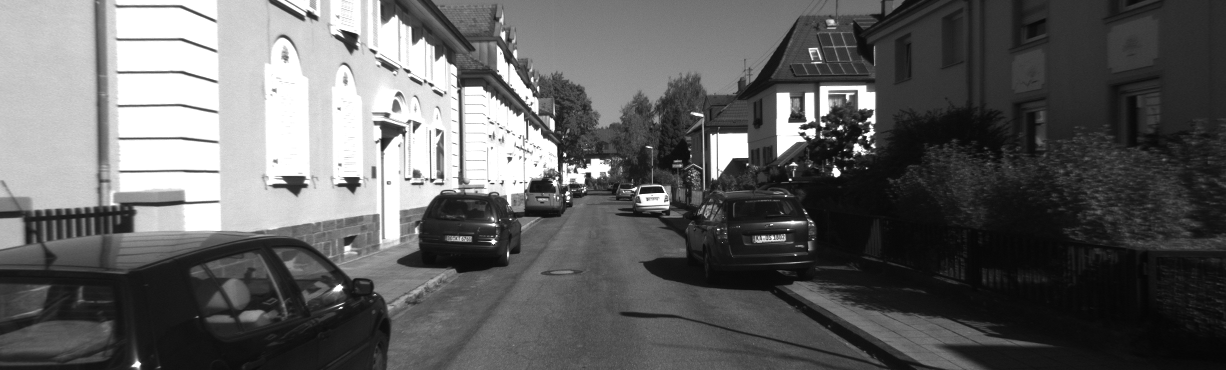
\includegraphics[width=0.75\textwidth]{imagenes/67_img0.png} } 

\subfloat[Imagen en escala de grises obtenida por la cámara derecha.]{
	\label{subfig:kitti-raw-1}
	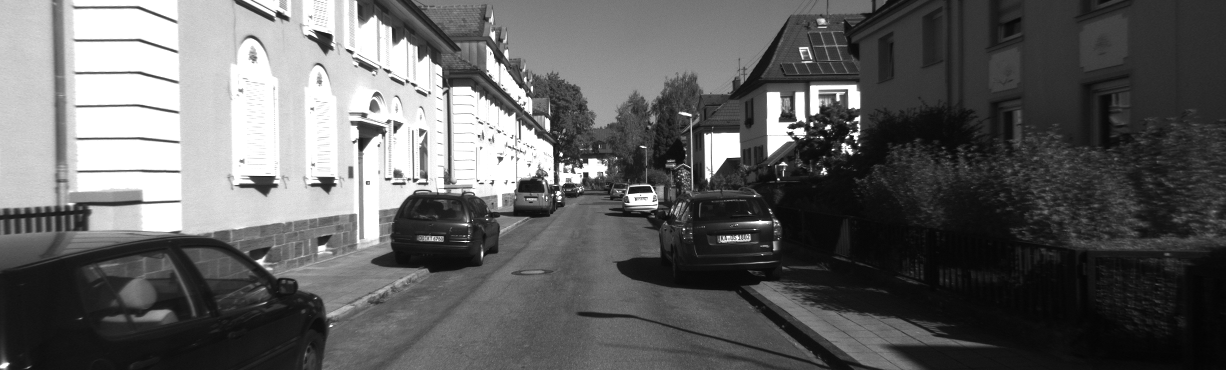
\includegraphics[width=0.75\textwidth]{imagenes/67_img1.png} } 

\subfloat[Imagen en color obtenida por la cámara izquierda.]{
	\label{subfig:kitti-raw-2}
	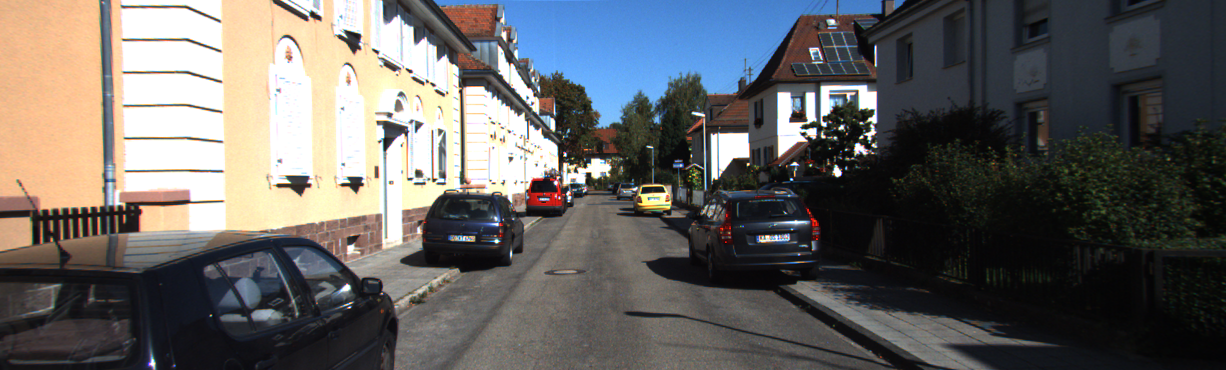
\includegraphics[width=0.75\textwidth]{imagenes/67_img2.png}} 

\subfloat[Imagen en color obtenida por la cámara derecha.]{
	\label{subfig:kitti-raw-3}
	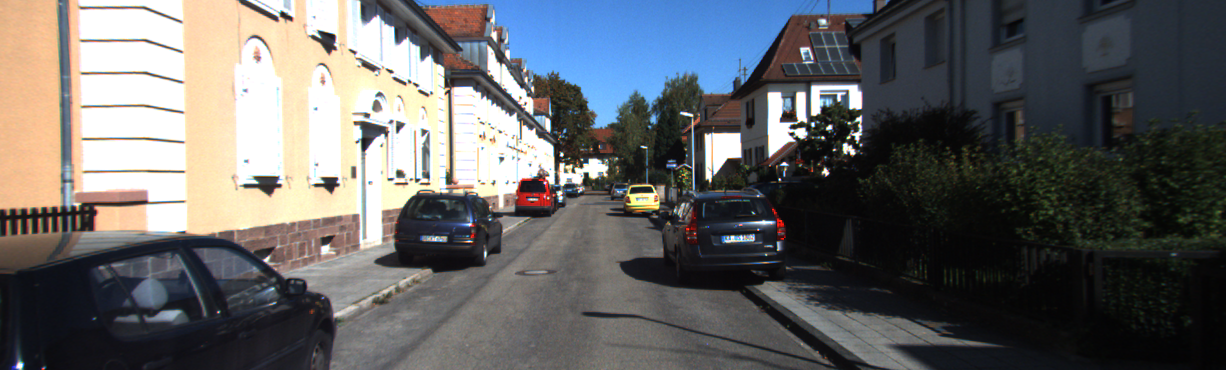
\includegraphics[width=0.75\textwidth]{imagenes/67_img3.png}}
	
\caption{Muestra de las cuatro imágenes en bruto disponibles en KITTI para un instante dado.}
\label{fig:kitti_raw}

\end{figure}

En total, se disponen de 192760 imágenes ($\sim$ 196 GB) de tamaño 1242x375 píxeles, de las cuales 96430 (la mitad) corresponden a las cámaras a color. Como el objetivo es la estimación de profundidades monocular, solo se emplea una de las imágenes de cada pareja de imágenes producido por el sistema de estereovisión, por lo que realmente se emplean 48215 imágenes (una cuarta parte de la cantidad original).

\subparagraph{Anotaciones}\mbox{}\\
Por otro lado, KITTI proporciona también imágenes formadas por los valores numéricos de la profundidad para cada uno de los píxeles de las imágenes presentadas previamente. Estos valores son los obtenidos por el escaner láser equipado en el vehículo, y por lo tanto pueden considerarse una medida fiable de la profundidad en cada imagen. Estas imágenes de profundidad serán las que se emplearan como anotaciones y por lo tanto, los valores que se emplearan para entrenar el modelo y evaluar su capacidad de predicción. Un punto importante a considerar sobre las medidas de estas anotaciones es que debido a la naturaleza del sensor con el que fueron tomadas, son anotaciones \textbf{dispersas} (\textit{sparse}) y no densas. Esto significa que no todos los píxeles de una imagen dada tienen anotación, y por lo tanto, aquellos píxeles no anotados deberán ser ignorados tanto durante el entrenamiento como durante la evaluación. Una muestra de estas etiquetas y de las anotaciones dispersas puede observarse en la Figura \ref{fig:kitti_depth}. Estas anotaciones están disponibles tanto como para las imágenes capturadas con las cámaras derechas como para las capturadas con las cámaras izquierdas, es decir, hay dos anotaciones para cada instante.

\begin{figure}[H]
\centering
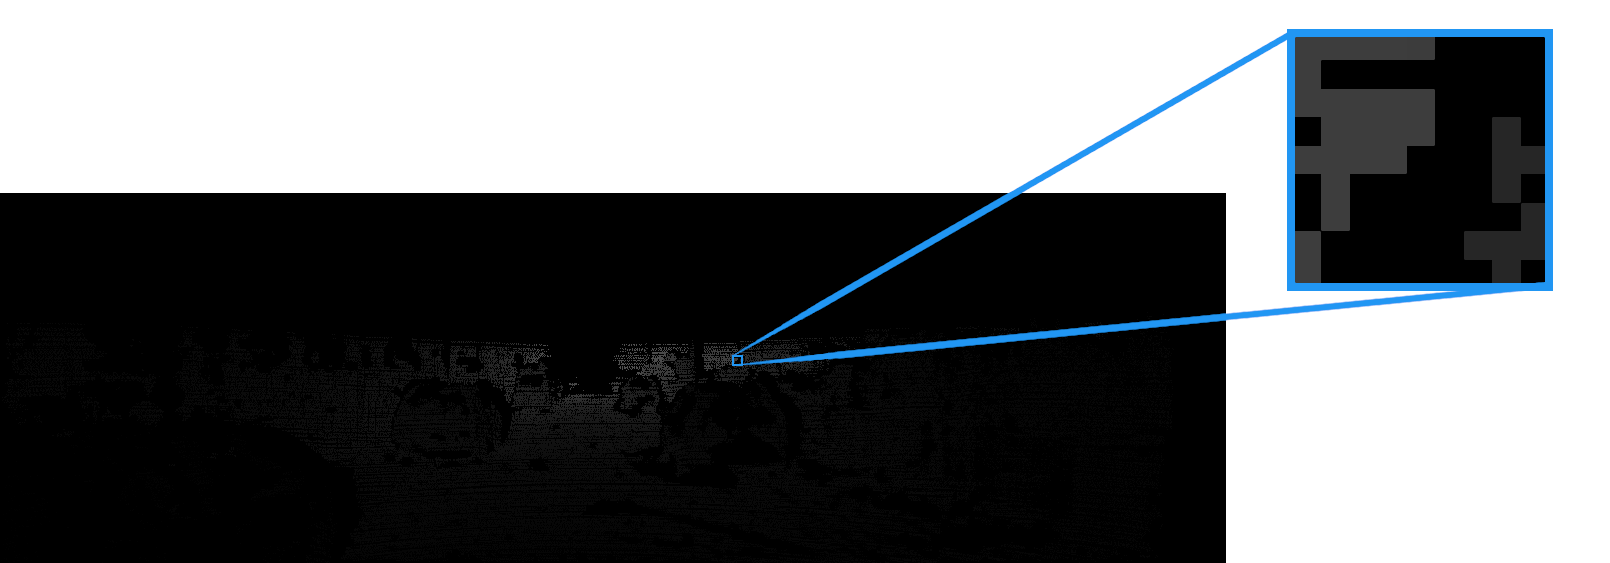
\includegraphics[width=\textwidth]{imagenes/depth67_img3_detail.png}
\caption{Anotación de KITTI y detalle de su carácter disperso para un instante dado.}
\label{fig:kitti_depth}

\end{figure}


\todo[inline]{Hablar de los datos que proporciona kitti}

\todo[inline]{Hablar de los splits de kitti y de la limpieza que se ha llevado a cabo}















\subsection{Arquitectura y capas}
Hablar de la arquitectura en concreto que se ha utilizado (DPT) apoyándose en todo lo que se haya explicado en el fundamento teórico. Explicar también las capas de atención que se han empleado en más detalle.

\subsection{Warmstart}
Hablar de que se ha hecho finetuning en vez de entrenar desde cero por las limitaciones de computo y de disponibilidad de datos. Aunque no todas las capas coincidiesen, se han empleado los pesos entrenados en general, NO los finetuneados ya en sus respectivos datasets (Esto en realidad estaría bien probarlo a ver si no hace mucho overfitting).

\subsection{Función de pérdida}
Hablar de la función de pérdida empleada para entrenar, hay que ver como se puede hilar esto con una sección en el fundamento teórico donde se expliquen más funciones de pérdida para estimación de profundidades.

\subsection{Data augmentation}
Hablar de data augmentation si se lleva a cabo, exponer las operaciones y justificarlas con regularización y generalización a casos nuevos, evitar que siempre se itere sobre las mismas imágenes.

\subsection{Evaluación}
Explicar el proceso de evaluación, justificar que como las redes grandes se han entrenado por los autores para trabajar con imágenes grandes y que nosotros estamos reduciendo su tamaño en la entrada, para la evaluación final en el conjunto de test se hacen grandes y así tener las mismas métricas. Hablar también de los recortes.

Explicar o aquí o en el dataset que se utiliza el conjunto de test, ni el de entrenamiento ni el de validación y justificarlo.

Meter aquí el apartado de métricas que se ha llevado a cabo.

Mencionar que las pruebas se llevaran a cabo en distintos entornos y que esto se señalará en los resultados.

Apuntar como se hace para estimar la profundidad métrica en un dataset concreto (aquí o en el apartado de arquitectura).

\subsection{Portabilidad (?) de los modelos}
Explicar el proceso que se ha llevado a cabo con onnx y por qué se emplea, explicar que hace onnx por debajo, hacer diagramas. Puede que esto colapse con la sección de software de arriba, se puede quitar.

% En los resultados hablar de la distribución de los pesos antes y después de convertir el modelo si es pertinente, hacer una especie de estudio de ablación si se puede entrenar modelos, etc. Puede estar interesante quitar cabezas de atención, quitar bloques de atención, ver como afecta al tamaño dle modelo, su rendimiento (velocidad y métricas)...

\clearpage
\section{Resultados}

Hablar de resultados cuantitativos (tablas con las métricas en distintas pruebas) y cualitativos (imágenes resultado de cada una de las pruebas - escaladas si es necesario - con el ground truth y con la imagen real de referencia). Mencionar que para que se vean mejor las imágenes los valores se han hecho relativos para así ocupar toda la escala de grises.

\clearpage
\section{Discusión}

Hablar y comentar los resultados obtenidos con otros resultados (convolucionales? y transformers), si los resultados en la jetson son lentos y no se puede acceder a otra más potente, buscar referencias para ver el incremento de rendimiento que presentan con otros algoritmos para poder dar una estimación de cuanto más rápido podría ir en otro hardware embebido más potente.

Mencionar que las capas eficientes no afectan muchisimo debido a que el tamaño de las cadenas de tokens no son demasiado grandes (estamos trabajando con imágenes pequeñas y no con larguisimas cadenas de texto para las que fueron diseñadas).

\clearpage
\section{Conclusiones y lineas futuras}
Overview del trabajo y de los resultados obtenidos, hacer hincapié en los modelos producidos y su utilidad, hablar del interés de la gente en optimizar este tipo de modelos (github)...


Decir que queda pendiente probar en otro hardware empotrado, entrenar con más datos, reentrenar desde cero sin hacer warmstart, entrenar en imagenet antes las transformers con las capas de atención modificadas, explorar más técnicas de optimización que no se han empleado, más atenciones efificnetes, aplicarlo a imágenes mucho mayores. Por otro lado, desarrollar aplicaciones con los modelos producidos como hacer un slam monocular, conducción autónoma, 

\end{document}